\chapter{Applications when you have one network}
\label{sec:ch7}

Over the last few chapters, we've come quite a long way. We've learned about network-valued data, and the intricacies of networks that make them unique. We've covered ways to conceptualize network-valued data, and how to capture the randomness inherent in network measurements using statistical models. Most recently, you learned a variety of approaches to take your network, and transform the network or collection of networks into a different representation. These representations offered the advantage of substantially reducing the complexity of the dependencies in network data, and in many cases, placed the network into a structure that you can deal with using traditional machine learning approaches. In this section, we'll begin to learn why, exactly, we transformed the network(s) into new representations. We'll cover machine learning systems that we can use, in conjunction with these new representations, to derive insights about our network(s). In some cases, we'll learn how to take what we learn about the network, and make general inferences that apply beyond just the particular network measurement we obtained. In this section, we'll cover how to do this when you have one network.

\begin{figure}[h]
    \centering
    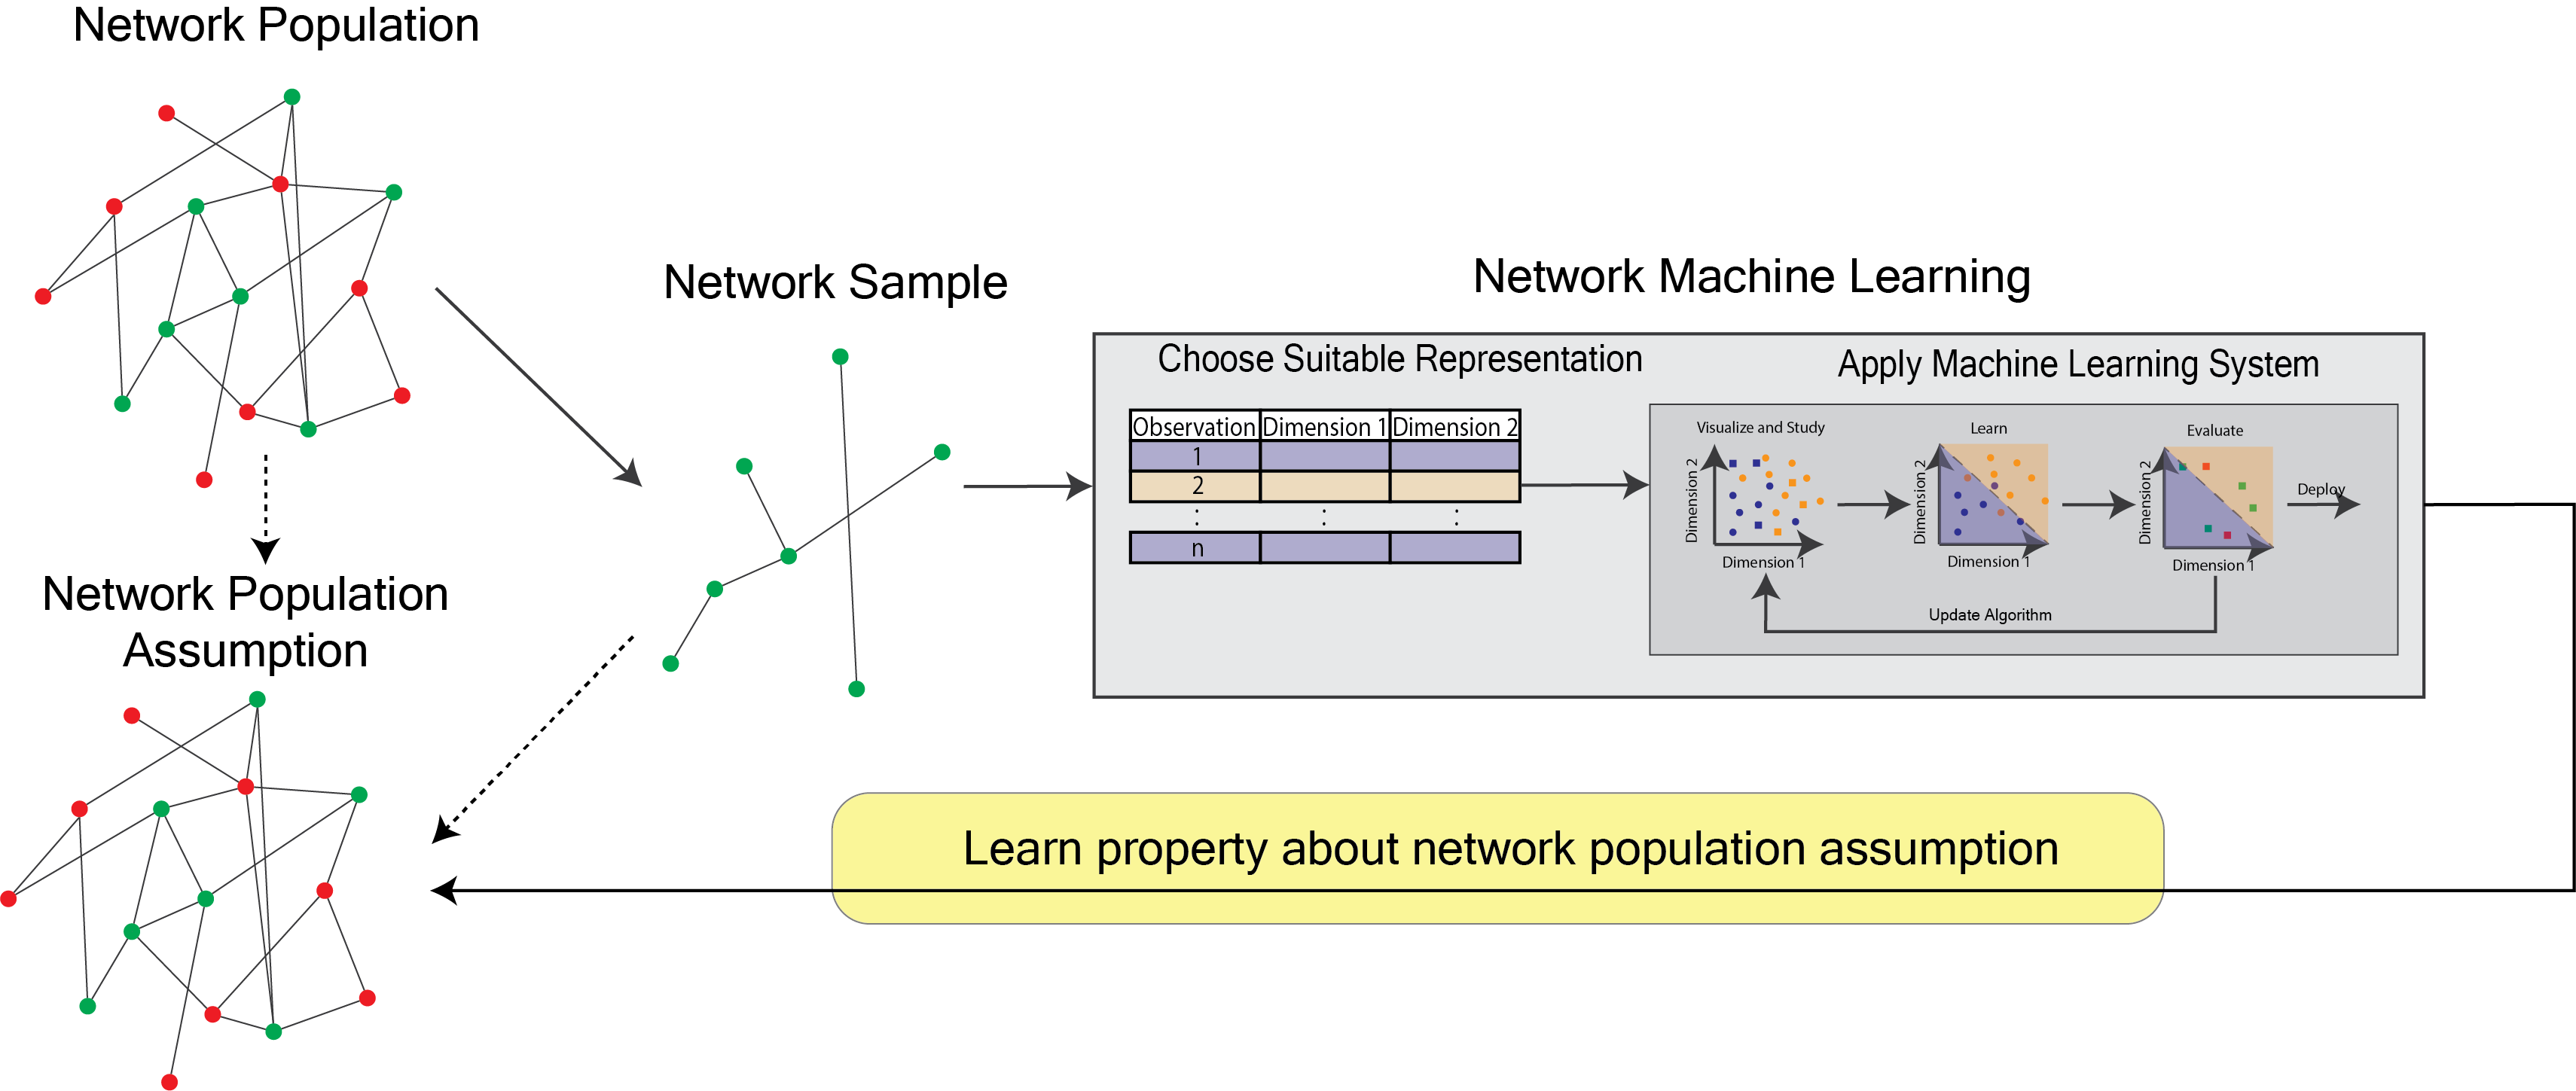
\includegraphics[width=\linewidth]{applications/ch7/Images/applications.png}
    \caption[Network machine learning applications schematic]{The statistical learning pipeline. In this chapter, you will learn about how to apply network machine learning systems to derive insights about a single network and its representation, and how to apply those insights to make inferences about the underlying network population.}
    \label{fig:ch7:netapps}
\end{figure}

\begin{comment}
\begin{enumerate}
    \item Section \ref{sec:ch7:comm_detect} introduces the community detection problem, and how we can use network embeddings to impute community labels for our network.
    \item Section \ref{sec:ch7:testing} details how we can test whether groups of edges differ in the network.
    \item Section \ref{sec:ch7:modelselect} covers how we can determine appropriate levels of model complexity for our network.
    \item Section \ref{sec:ch7:vn} introduces the vertex nomination problem, which allows us to find nodes that are ``similar'' to reference nodes.
    \item Section \ref{sec:ch7:oos} indicates how we can embed new nodes into an existing network embedding.
\end{enumerate}
\end{comment}
\newpage

\section{The community detection problem}
\label{sec:ch7:comm_detect}

Throughout most of this book to date, when dealing with stochastic block models, we've assumed that we knew the community assignments ahead of time. As you learned in Section \ref{sec:ch5:psd_block:same_lp}, with networks that have an underlying block-like structure, the underlying latent positions were equal (up to a possible re-scaling by a degree-correction factor) for all nodes in the same commmunity.

When we used \texttt{ase} or \texttt{lse} to embed positive semi-definite probability matrices (and more generally, any probability matrix) in Section \ref{sec:ch6:ase} and \ref{sec:ch6:lse}, we could obtain reasonable estimates of the underlying latent position matrices (up to a rotation). We asserted, without much to back it up, that this ``latent representation'' of the adjacency matrix as a tabular structure would allow us to learn latent patterns in our network that might not necessarily be obvious at first glance which, therefore, greatly simplified the conceptually complicated dependency structures that existed in our adjacency matrix. 

Let's revisit a version of our working example from Section \ref{sec:ch6:lse}, which was a network sampled from a homophilic $DCSBM_n(\vec z, \vec\theta, B)$ random network, but which has three communities instead of two. We'll also reorganize the nodes of the matrix randomly like we did in Section \ref{sec:ch6:ase:reorder}, since in many networks that you obtain, you might not be spoon-fed nodes that are pre-ordered to reflect the community structure:

\begin{lstlisting}[style=python]
import numpy as np
from graphbook_code import dcsbm

nk = 100  # 100 nodes per community
K = 3  # the number of communities
n = nk * K  # total number of nodes

zs = np.array([k for k in range(1, K + 1) for i in range(nk)])
# block matrix and degree-correction factor
B = np.array([[0.6, 0.2, 0.1], [0.2, 0.4, 0.1], [0.1, 0.1, 0.3]])
theta = np.tile(np.linspace(0, 1, nk), K)
# generate network sample
A = dcsbm(zs, theta, B)

# permute the nodes randomly
vtx_perm = np.random.choice(n, size=n, replace=False)
Aperm = A[tuple([vtx_perm])] [:,vtx_perm]
zperm = np.array(zs)[vtx_perm]
\end{lstlisting}
The network probability matrix is shown in \ref{fig:ch7:comm_detect:ex}(A), and the adjacency matrix is shown in Figure \ref{fig:ch7:comm_detect:ex}(B). Looking at the adjacency matrix, there is no obvious structure to the network.

\begin{figure}[h]
    \centering
    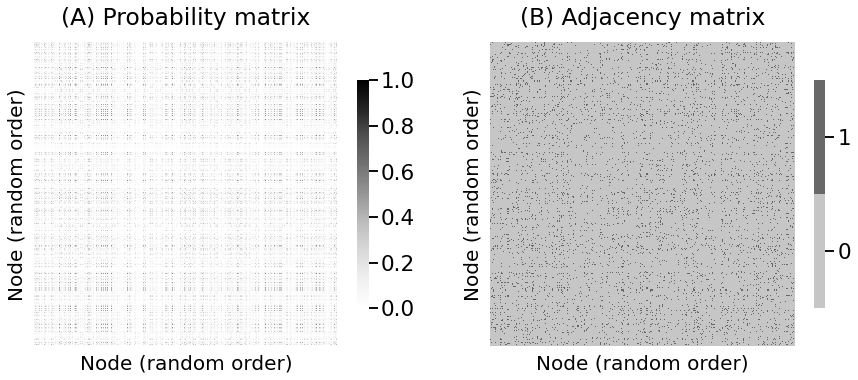
\includegraphics[width=\linewidth]{applications/ch7/Images/comm_detect_ex.png}
    \caption[Community detection three community example]{\textbf{(A)} the probability matrix for the $DCSBM_n(\vec z, \vec \theta, B)$ random networks, and \textbf{(B)} a sample of the random network.}
    \label{fig:ch7:comm_detect:ex}
\end{figure}
We encourage you to go through the procedure of making a histogram of the node degrees to observe that the network appears to be slightly heavy-tailed, which would encourage the use of \texttt{lse}. However, for the purposes of this section, we will proceed with \texttt{ase}, as we will adjust for the elliptical-shaped latent positions using a different strategy later on. 

\begin{floatingbox}[h]\caption{Refamiliarize yourself with unsupervised learning}
In this next section, we will assume that you are familiar with several concepts from unsupervised learning, including the $k$-means algorithm, the Adjusted Rand Index (ARI), confusion matrices, and the silhouette score. If you aren't already familiar or want a quick refresher, check out the unsupervised learning basics section of the appendix in Appendix \ref{app:ch14:unsup}, which covers the required background knowledge for these concepts.

Briefly, we will use $k$-means to estimate the latent community assignment vector, the ARI and confusion matrices to study the homogeneity of the resulting latent community estimates, and the silhouette score to evaluate the latent community estimates.
\end{floatingbox}

\subsection{Spectral clustering with a pre-defined number of communities}
\label{sec:ch7:comm_detect:known}

When you embed a network with a defined number of communities, remember to equate the number of embedding dimensions with the number of communities, because the true latent position matrix has one latent dimension for each community as you learned in Section \ref{sec:ch5:psd_block:same_lp}. In this case, since $K=3$, we embed with $3$ embedding dimensions:

\begin{lstlisting}[style=python]
import scipy as sp
from graspologic.embed import AdjacencySpectralEmbed as ase

Xhat = ase(n_components=3).fit_transform(Aperm)
D = sp.spatial.distance_matrix(Xhat, Xhat)
\end{lstlisting}
We plot the second and third embedding dimensions as a scatter plot in Figure \ref{fig:ch7:comm_detect:embed}(A), but we would encourage you to look at the entire pairs plot. Note that even though the nodes in \texttt{Aperm} were completely randomized, the estimated latent positions still retain a ``blob'' structure, where groups of nodes in the same community look spatially quite close to one another. This is reflected in the distance matrix in Figure \ref{fig:ch7:comm_detect:embed}(B), where we can see that the within-community pairwise distances tend to be less than the between-community pairwise distances.


\begin{figure}[h]
    \centering
    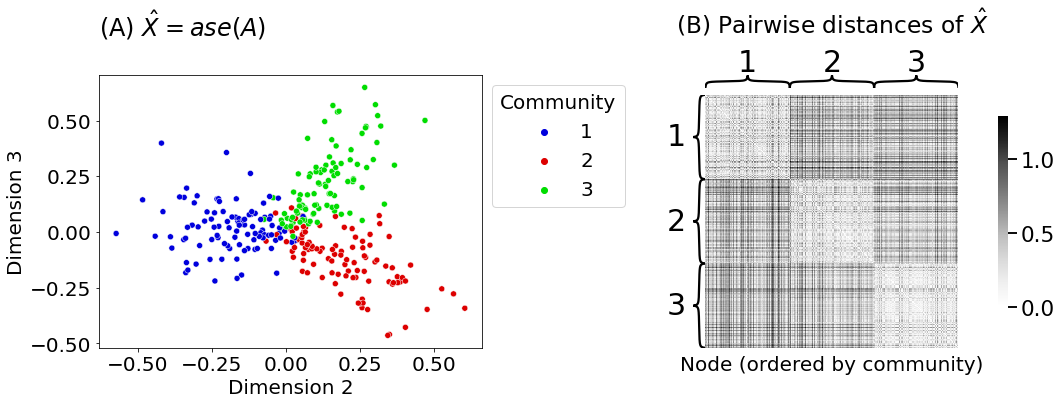
\includegraphics[width=\linewidth]{applications/ch7/Images/comm_detect_embed.png}
    \caption[Community detection spectral embedding and pairwise distances]{\textbf{(A)} a spectral embedding of the randomly ordered adjacency matrix. \textbf{(B)} the pairwise distances between the estimated latent positions for each pair of nodes.}
    \label{fig:ch7:comm_detect:embed}
\end{figure}

\subsubsection{Estimating community assignments via \texttt{KMeans}}

First, we use \texttt{KMeans} to estimate the latent community assignment vector, which we will denote with $\hat{\vec z}$. Remember that $\hat\cdot$ just means an estimate: in this case, an estimate of the community assignment vector $\vec z$ for an underlying $DCSBM_n(\vec z, \vec \theta, B)$ random network. We can produce the estimate of the community assignment vector using \texttt{KMeans()} from \texttt{sklearn}:

\begin{lstlisting}[style=python]
from sklearn.cluster import KMeans

labels_kmeans = KMeans(n_clusters = 3).fit_predict(Xhat)
\end{lstlisting}

One slight problem with this procedure is that, by being fully unsupervised, there is no reason that the labels that we estimate will necessarily ``align'' with true descriptors (such as communities) with the nodes. For instance, in this case, we have no reason to believe, for instance, that community $1$ produced by \texttt{KMeans} will necessarily correspond to community $1$ in our network. For this reason, we need to get a bit creative when evaluating unsupervised clustering techniques.

\paragraph{Evaluating your clustering}
\label{ch7:comm_detect:eval}

In this instance, true-community labels are already known, because this is just a simulation. When you know true node labels ahead of time, you can do some special evaluations that take advantage of the fact that you have the true labels. The first of these is to study the confusion matrix, which you can produce with \texttt{sklearn}'s \texttt{confusion\_matrix()}:

\begin{lstlisting}[style=python]
from sklearn.metrics import confusion_matrix

# compute the confusion matrix between the true labels z
# and the predicted labels labels_kmeans
cf_matrix = confusion_matrix(zperm, labels_kmeans)
\end{lstlisting}

The confusion matrix is shown in Figure \ref{fig:ch7:comm_detect:eval}(A). You will see that when you have a clustering that aligns well with your true labels, the predictions will tend to be homogeneous: a particular true label will correspond to a particular predicted label, and vice-versa. You can evaluate this homogeneity (how well, in general, one true label corresponds to one predicted label, and vice-versa) using the Adjusted Rand Index (ARI), where a score of closer to $1$ indicates that the true and predicted labels are perfectly homogeneous (one true label corresponds to exactly one predicted label):

\begin{figure}[h]
    \centering
    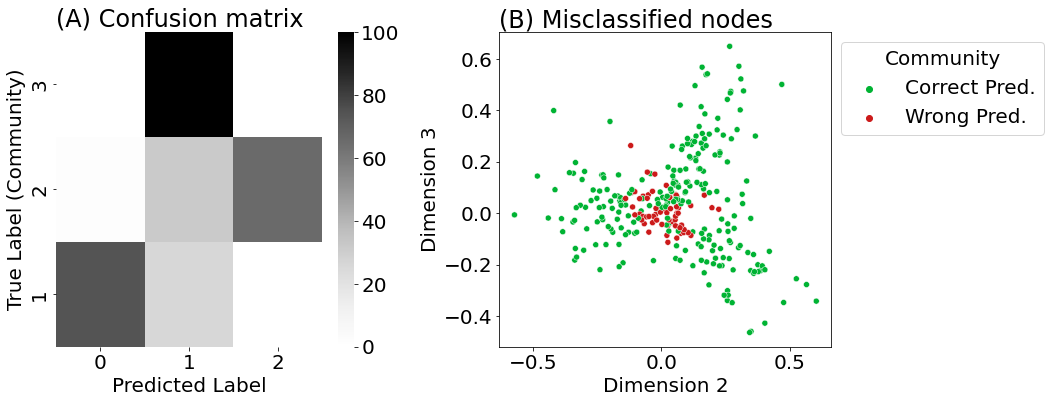
\includegraphics[width=\linewidth]{applications/ch7/Images/comm_detect_eval.png}
    \caption[Community detection clustering evaluation]{\textbf{(A)} the confusion matrix. \textbf{(B)} the estimated latent positions, along with whether the node was classified correctly (or not) after realigning the predicted communities with the true communities.}
    \label{fig:ch7:comm_detect:eval}
\end{figure}

\begin{lstlisting}[style=python]
from sklearn.metrics import adjusted_rand_score

ari_kmeans = adjusted_rand_score(zperm, labels_kmeans)
print(ari_kmeans)
# 0.4687
\end{lstlisting}
This score of about $0.5$ indicates that the predicted communities tend to be relatively homogeneous with the true labels, but the clustering is imperfect.


\paragraph*{By remapping the labels, we can evaluate the error rate}

Looking back at the confusion matrix in Figure \ref{fig:ch7:comm_detect:eval}, it looks like we have a reasonable pattern we can establish:
\begin{enumerate}
    \item Nodes that are assigned a predicted label of $0$ tend to correspond to community $1$, 
    \item Nodes that are assigned a predicted label of $1$ tend to correspond to community $3$, and
    \item Nodes that are assigned a predicted label of $2$ tend to correspond to community $2$.
\end{enumerate}
It seems clear that this would make for a reasonable \textit{correspondence} between the predicted and true labels. A \textit{correspondence} between two sets (in this case, the predicted and true labels for node communities) refers to the fact that we can define a mapping that relates the elements of the predicted labels to the true labels. 

Results that are not as homogeneous as they are here can be quite finnicky, so we will avoid going into too much depth in this book. We can remap the labels with \texttt{graspologic}'s \texttt{remap\_labels()} utility:

\begin{lstlisting}[style=python]
from graspologic.utils import remap_labels

labels_kmeans_remap = remap_labels(zperm, labels_kmeans)
\end{lstlisting}
With the labels from \texttt{KMeans} properly aligned to the true community labels, we can evaluate the error rate of our function. You can do this with \texttt{numpy} like this:

\begin{lstlisting}[style=python]
# compute which assigned labels from labels_kmeans_remap differ from the true labels z
error = z - labels_kmeans_remap
# if the difference between the community labels is non-zero, an error has occurred
error = error != 0
er_rt = np.mean(error)  # error rate is the frequency of making an error
\end{lstlisting}

In Figure \ref{fig:ch7:comm_detect:eval}(B), we visualize the misclassified points as a function of the data matrix that is being leveraged to estimate community assignments, the estimated latent position matrix. Notice that we do a good job of classifying points in the ``arms'' of the individual blobs of nodes (the \textit{clusters}), but tend to do worse for the points that are located between the clusters of nodes. This happens because of the manner in which predicted community labels are applied by \texttt{KMeans}. See Remark \ref{box:ch7:kmeans_for_sc} and Appendix \ref{app:ch14:unsup} for more detailed commentary about why this happens.

\begin{floatingbox}[h]\caption{Why does \texttt{KMeans} perform well for clustering samples of block models?}
\label{box:ch7:kmeans_for_sc}
When we cluster points using \texttt{KMeans}, remember that we will tend to identify clusters which reflect blobs of points in our data which have similar pairwise distances (which, in most cases, will be the pairwise Euclidean distance). Points are assigned to the cluster that they are closest to, and as the \texttt{KMeans} algorithm iterates, it attempts to identify cluster centers which minimize the cumulative pairwise distance from each pair of points to the nearest cluster. 

\,\,\,\, Remember from Section \ref{sec:ch5:psd_block:same_lp} that with stochastic block models, the underlying latent positions are identical. As we learned in Section \ref{sec:ch6:ase} the estimated latent positions tend to ``approximate'' the true latent positions. The estimates will retain this feature and the estimated latent positions will be similar (in terms of their Euclidean distance) if they are in the same community for the stochastic block model, and will tend to materialize as relatively sphere-shaped ``globs'' in the estimated latent positions. 
\end{floatingbox}

In the case of the degree-corrected stochastic block model, the underlying latent positions are identical up to a rescaling along the direction of the community-specific latent position vector. This will tend to materialize as relatively elliptical-shaped globs in the estimated latent positions along the direction of the rescaling in the underlying community-specific latent position vector. This is undesirable when we try to cluster, because \texttt{KMeans} is effectively ``penalizing'' a difference between a point and the community center symmetrically in Euclidean space. In reality, we would want the ``penalty'' to be applied asymmetrically. This motivates the use of clustering techniques which are more adaptive to rescalings along the community-specific latent position vectors, such as \texttt{GMM}, as degree heterogeneity is a common problem encountered in network data. You can explore this more in-depth by completing the exercise in Remark \ref{box:ch7:gmm}.

\begin{floatingbox}[h]\caption{Using \texttt{GMM} for clustering samples of block models}
\label{box:ch7:gmm}
Simulate from a $DCSBM_n(\vec z, \vec \theta, B)$ random network, like we did above, but skew the degree-correction vector more dramatically, with $K=2$ communities. 
\begin{enumerate}
    \item Spectrally embed the adjacency matrix into two dimensions, and illustrate that the estimated latent positions appear to be elliptical.
    \item Apply \texttt{GMM} to cluster the estimated latent positions, using \texttt{GaussianMixture} from \texttt{sklearn}. Use the techniques that we described here to evaluate the clustering procedure.
    \item Plot the community centers (the \texttt{means\_} attribute of the instantiated class) estimated by \texttt{GMM}, and plot ellipses reflecting the estimated covariance (the \texttt{covariances\_} attribute) about the community centers. You can do this by following the tutorial \cite{sklearngmm_tut}.
    \item For each point in the network, compute the probability that the point is from its assigned cluster, using the \texttt{predict\_proba()} function from the \texttt{GaussianMixture} object. Plot the estimated latent positions, with the color going from low probability (red) to high probability (green).
\end{enumerate}
Use the objective function for \texttt{GMM} to argue that this result supports that \texttt{GMM} tends to penalize points less if they are farther away from the community center but along the principal axis of the community-specific ellipse, and more if they are farther away from the community center but not along the principal axis of the community-specific ellipse. Argue why this makes sense in the context of the $DCSBM_n(\vec z, \vec \theta, B)$ random network underlying your network sample by discussing the degree-correction factor heterogeneity.
\end{floatingbox}

\subsection{Spectral clustering with an undefined number of communities}
\label{sec:ch7:comm_detect:unknown}

In real data, you almost never have a beautiful canonical modular structure that makes choosing a number of communities obvious. Further, by applying unsupervised clustering algorithms in the first place and attempting to learn community labels from your data, it's likely that you wouldn't know reasonable community labels that you would expect to obtain going in. This means that it is extremely infrequently going to be the case that you know exactly how you should set the number of communities, $K$, or the number of embedding dimensions ahead of time.

\begin{floatingbox}[h]\caption{Nomenclature about clusters and communities}
With unsupervised classification, groups of points that are assigned to the same group by the trained classifier are typically called a ``cluster''. However, in our case, they are more than just clusters: they are predicted node community labels. For this reason, when we are referring specifically to the assignments themselves, we will often refer to this concept as ``predicted communities'' or something of the like. When we are referring to ``blobs of points'', we will often default to calling them clusters of points. 
\end{floatingbox}

The procedure for estimating the community assignment vector is similar to the one we used previously in Section \ref{sec:ch7:comm_detect}. We again embed, but this time because we don't know the number of communities we are looking for, we will use automatic elbow selection from Section \ref{sec:ch6:dimest:dimselect}:

\begin{lstlisting}[style=python]
Xhat = ase().fit_transform(Aperm)
print("Estimated number of dimensions: {:d}".format(Xhat.shape[1]))
# Estimated number of dimensions: 3
\end{lstlisting}
Examining the pairs plot, we would again find that Dimensions 2 and 3 (as before) show fairly clearly stratified blobs in the estimated latent positions, in Figure \ref{fig:ch7:comm_detect:embed}(A). 

Since we do not know the optimal number of communities $K$ nor the true community assignments, we must choose an unsupervised clustering technique which allows us to compare clusterings with different choices of community counts. Fortunately, this is pretty easy for us to do, too, using a simple statistic known as the silhouette score, which is described in Appendix \ref{app:ch14:unsup:eval:silhouette}.

\subsubsection{Using the silhouette score to deduce an appropriate number of communities}

Using the silhouette score, deducing an appropriate number of communities is pretty easy. We choose a range of communities that we think might be appropriate for our network. Let's say, for instance, we think there might be as many as $10$ communities in our dataset. We perform a clustering using unsupervised learning for all possible numbers of communities, from $2$ all the way up to the maximum number of communities we think could be reasonable. Then, we compute the silhouette score for each number of communities. Finally, we choose the number of communities that has the highest Silhouette score. 

Let's see how to do this, using \texttt{graspologic}'s \texttt{KMeansCluster()} function:

\begin{lstlisting}[style=python]
from graspologic.cluster import KMeansCluster

km_clust = KMeansCluster(max_clusters = 10)
km_clust = km_clust.fit(Xhat)
\end{lstlisting}

To determine an optimal number of clusters, we can visualize the silhouette score as a function of the number of clusters:

\begin{lstlisting}[style=python]
import seaborn as sns
from pandas import DataFrame as df

nclusters = range(2, 11)  # graspologic nclusters goes from 2 to max_clusters
silhouette = km_clust.silhouette_ # obtain the respective silhouettes

# place into pandas dataframe
ss_df = df({"Number of Communities": nclusters, "Silhouette Score": silhouette})
sns.lineplot(data=ss_df, x="Number of Communities", y="Silhouette Score")
\end{lstlisting}

In Figure \ref{fig:ch7:comm_detect:kmclust}(A), we look at the number of communities as a function of the silhouette score. Notice that \texttt{KMeans} with silhouette score analysis determines that the optimal number of communities is $\hat K = 4$. 

Figure \ref{fig:ch7:comm_detect:kmclust}(B) shows the predicted communities for each node coloring the estimated latent dimensions. It appears that \texttt{KMeans} has been ``fooled'' by the elliptical, non-spherical embeddings, and in fact determined optimal unsupervised classification performance could be achieved by adding a fourth community to the center of the estimated latent positions. This is because \texttt{KMeans} and the silhouette score penalize all dimensions equally, which as you found in Remark \ref{box:ch7:gmm}, might not always be desirable. 

\begin{figure}[h]
    \centering
    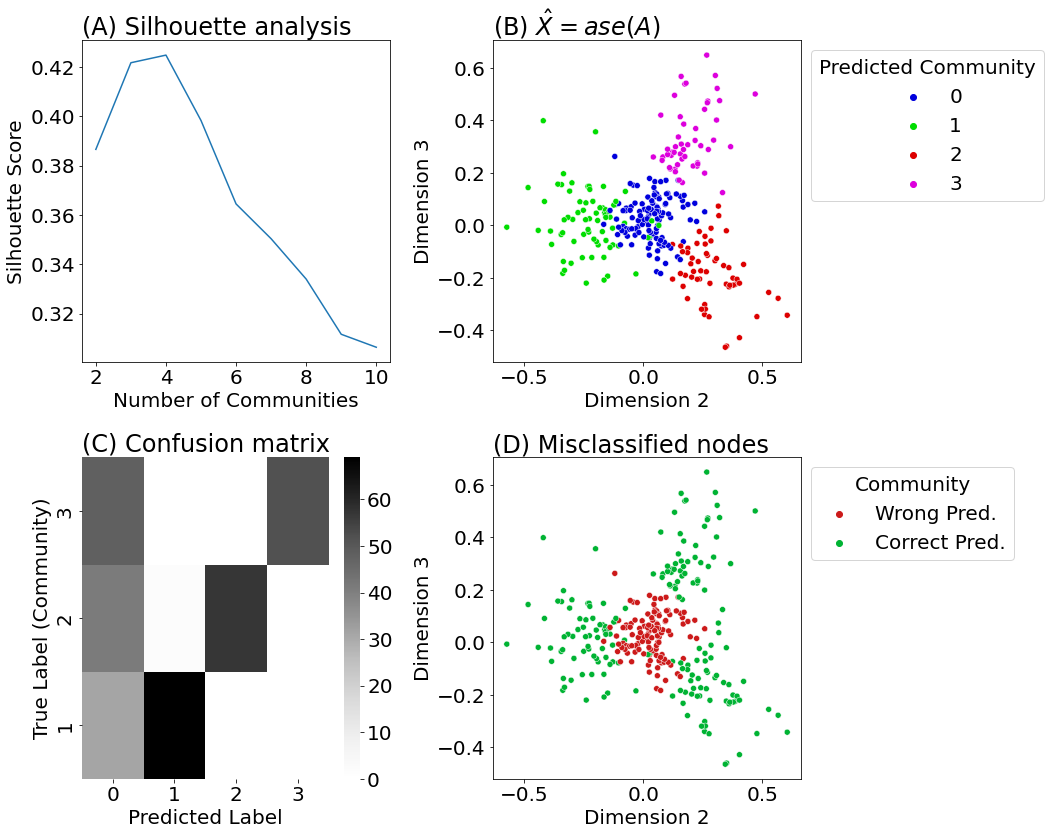
\includegraphics[width=\linewidth]{applications/ch7/Images/comm_detect_kmclust.png}
    \caption[Unsupervised community detection without knowing number of communities]{\textbf{(A)} an analysis of the silhouette scores as a function of the number of communities. \textbf{(B)} the predicted communities for each node. \textbf{(C)} the confusion matrix with $\hat K = 4$. \textbf{(D)} the misclassified points.}
    \label{fig:ch7:comm_detect:kmclust}
\end{figure}


\paragraph*{Determining what the predicted communities correspond to}

We plot the confusion matrix as a function of the true node community in Figure \ref{fig:ch7:comm_detect:kmclust}(C). The ``arms'' of the ellipses in Figure \ref{fig:ch7:comm_detect:kmclust}(B) correspond to predicted labels of $1$ through $3$ respectively, and nearly perfectly correspond with the true underlying node communities $1$ through $3$ respectively in Figure \ref{fig:ch7:comm_detect:kmclust}(C). On the other hand, the $0$ community at the center of the arms does not correspond to any specific true label particularly well, and is an agglomeration of points at the bases of the arms across all three true communities. We visualize the points that are misclassified in Figure \ref{fig:ch7:comm_detect:kmclust}(D), which correspond to the points assigned to the $0$ community. 

\paragraph*{The art of determining what predicted communities mean}

By now, you know how to apply spectral clustering to network data and evaluate it when you have a single node covariate (in this case, the true node communities). However, real data are not nearly this cut and dry: typically, associated with each node, you may have many covariates, some of which might not even have discrete (one of $K$) labels. For instance, in Figure \ref{fig:ch2:brain_preds}, for each node we had a spatial position, which would not be very easy to interpret our communities on the basis of.

For this reason, there is quite an art to determining what predicted communities mean, much like many other applications of unsupervised learning in machine learning more generally. You may have to take features that describe your nodes, such as the spatial positions listed above, and take functions of these spatial positions (such as determining the lobe of the brain that the spatial position falls into, which we described as a possible route we could take in Section \ref{sec:ch2:discover}) to be able to obtain a sensible understanding of what the communities correspond to. 

In many contexts, you might not even know what these communities correspond to at all, and you might have to rethink how the network was collected and work from the ground up to try to find meaning in the predicted communities. In this sense, once you perform community detection and identify stable communities that appear to be well-separated, your role as a network learning scientist has really just started.

\subsection{Extending community detection to other formulations}

Algorithm \ref{alg:ch7:sc} provides a generic formulation of the community detection process for network data with adjacency representations using \texttt{KMeans} and \texttt{ase}. Note that the procedures we detail generalize readily to alternative approaches in which the network data can be represented as a matrix. 

\begin{algorithm}[h]
\caption{Unsupervised  spectral community detection from network data with \texttt{KMeans}}
\label{alg:ch7:sc}
\KwData{$A$ the adjacency matrix of your network.\newline $d$ Optionally, a number of embedding dimensions.\newline $K$ Optionally, a number of communities.}
\KwResult{predicted community assignments.}
\SetAlgoLined

Let $\hat X = \texttt{ase}(A, d)$. If the dimensionality $d$ is unspecified, estimate it through elbow selection in Section \ref{sec:ch6:dimest:dimselect}.

Train a \texttt{KMeans} classifier, using the representation $\hat X$, to identify $K$ communities. If the number of communities is unspecified, evaluate the classifier over a range of reasonable numbers of communities, and evaluate the clusterings using a pre-defined evaluation metric. Represent this trained classifier as the community centers $\hat{\vec \mu}_k$ for each community $k$. 

For all points, compute $d_{ik} = \|\hat{\vec x}_i - \hat{\vec \mu}_k\|_2$, or the distance from each node $i$'s estimated latent position to the community center $k$, for all communities.

Let $\hat z_i = \text{argmin}_k d_{ik}$ be the predicted community for node $i$, which is the community corresponding to the center that is closest to the estimated node latent position for node $k$.

\Return{$\hat z$}
\end{algorithm}

For instance, we could substitute \texttt{lse} for \texttt{ase}, and potentially be more robust to degree variation in the network. If we had many networks with an underlying shared structure that we wanted to learn about, we could perform \texttt{mase} on our collection of networks, and use unsupervised learning techniques to learn about the underlying shared latent position matrix. If we had particular node covariates that we wanted to incorporate into our clustering, we could use \texttt{case} to embed a weighted combination of topological network structures with node-specific covariates, and produce communities that might meaningfully inform our ability to learn from our network data. Further, we could look to non-spectral embedding techniques as well to learn latent representations about our networks. We will discuss a few in Section \ref{sec:ch10:next}.

Finally, as we covered in Remark \ref{box:ch7:gmm}, there are many unsupervised learning techniques (such as \texttt{GMM}) that we could leverage to estimate community labels from our network. If you do not specify the number of communities ahead of time and wish to evaluate a range of possible numbers of communities, it is important that you choose evaluation criteria that will reflect your choice of clustering technique. As we noted in Remark \ref{box:ch7:gmm}, \texttt{GMM} gives us flexibility in terms of degree-heterogeneities that may materialize in our embeddings. These heterogeneities made the naive Euclidean distance potentially unsuitable if our communities that we expect in our network are elliptical. However, the evaluation criteria that we used for \texttt{KMeans} (the silhouette score) uses this same Euclidean distance, and therefore might run into similar issues if used as a metric for identifying a suitable number of communities. For this reason, there might be more appropriate evaluation metrics for the particular unsupervised learning technique that you identify. In \texttt{GMM}, for instance, a popular choice is number of communities that minimizes the \texttt{BIC}.




\newpage
\section{Sparsity}
\label{sec:ch7:sparse}

In Section \ref{sec:ch4:prop-net:density}, you learned about a very important descriptive property of networks called the network density. An understanding of the network density gives us the ability to describe another extremely ubiquitous property of networks: the network sparsity. 


To understand this section, we're going to use the working example in Remark \ref{box:ch7:sparse}:

\begin{floatingbox}[h]\caption{Sparse network example}
\label{box:ch7:sparse}
The nodes of the network will represent academic scholars in computer science from $K$ universities. For every university, there are $100$ scholars investigated for an arbitrary sample of researchers in the community. An edge exists if a pair of researchers have co-authored a paper together. Therefore, researchers who work with more people will have more edges, and consequently, a higher node degree.

Most researchers publish a lot of papers with their working groups; the within-university probability will be $1$, but the between-university probability will be $0.01$ (the network is extremely homophilic).

$95\%$ of the researchers will prot\'eg\'es; they are not yet running a lab, so most of their work occurs with close collaborators at their university. These researchers have a degree-correction factor that is $Beta(1, 4)$ distributed; this just means that their degree-correction factors will be between $0$ and $1$, but will tend to be quite low (on average, $\frac{1}{1 + 4} = \frac{1}{5}$). 

On the other hand, $5\%$ of the researchers will be lab leaders; they tend to spend a lot of time working with researchers both within and outside of their university. These researchers will have a degree-correction factors that is $Beta(2, 1)$ distributed; again this means the degree-correction factors will be between $0$ and $1$, but will tend to be quite high (on average, $\frac{2}{1 + 2} = \frac{2}{3}$).
\end{floatingbox}


We can produce our network like this, which is very similar to how we generated a $DCSBM_n(\vec z, \vec \theta, B)$ sample in Section \ref{sec:ch5:dcsbm}. We separate out the construction of the probability matrix here so that we don't have to sample the entire network every time, which gets very cumbersome:

\begin{lstlisting}[style=python]
import numpy as np
from graspologic.simulations import sample_edges
from graphbook_code import generate_sbm_pmtx
    
def academic_pmtx(K):
    """
    Produce probability matrix for academic example.
    """
    nk = 100
    n = K*nk
    # get the community assignments
    zs = [k for k in range(1, K + 1) for i in range(nk)]
    # randomly generate proteges and lab leaders
    unif_choices = np.random.uniform(size=n)
    thetas = np.zeros((n,))
    # 90% are proteges
    thetas[unif_choices > .1] = np.random.beta(1, 5, size=(unif_choices > .1).sum())
    # 10% are lab leaders
    thetas[unif_choices <= .1] = np.random.beta(2, 1, size=(unif_choices <= .1).sum())
    # define block matrix
    B = 0.01*np.ones((K, K))
    np.fill_diagonal(B, 1)
    # generate probability matrix for SBM
    Pp = generate_sbm_pmtx(zs, B)
    thetas = thetas.reshape(-1)
    Theta = np.diag(thetas)
    # adjust probability matrix for SBM by degree-corrections
    P = Theta @ Pp @ Theta.transpose()
    return P

def academic_example(K):
    P = academic_pmtx(K)
    return sample_edges(P)
\end{lstlisting}

First, we will introduce a few concepts about sparsity, and then we’ll tie in how this comes into play with learning from your network data. As a quick forenote, this section is going to assume that you have a working knowledge of the concept of a sequence, and that you have conceptualized algorithmic complexity and asymptotic notation at some point in your work life. If you need a quick refresher on asymptotic notation, we'd recommend that you give the wikipedia page a read-over \cite{bigonotation}. We summarized the big concepts that we will touch on in Remark \ref{box:ch7:asy}. Finally, we will see how the typical modes that network data are stored and analyzed can benefit if we know ahead of time that the network is sparse.


\begin{floatingbox}[h]\caption{Asymptotic notation}
\label{box:ch7:asy}
Asymptotic notation is a description of what happens at the limits of the domains of functions. Suppose that $f(x)$ and $g(x)$ are two functions, that are defined for real values $x$. Common asymptotic notations include:
\begin{enumerate}
    \item $f(x) = \mathcal O(g(x))$: ``$f(x)$ is big-O of $g(x)$'' means that $g(x)$ is a rate that upper-bounds $f(x)$. Formally, there exists a constant multiplier $M$ and a value $x_M$ where for any value $x \geq x_M$:
    \begin{align*}
        |f(x)| \leq Mg(x).
    \end{align*}
    The idea here is that $g(x)$ is an upper bound for $f(x)$ (for some arbitrary constant $M$).
    \item $f(x) = \smallO(g(x))$: ``$f(x)$ is little-o of $g(x)$'' means that for \textit{any} positive constant $\epsilon$, there exists an $x_\epsilon$ where for any value $x \geq x_\epsilon$:
    \begin{align*}
        |f(x)| \leq \epsilon g(x).
    \end{align*}
    The intuition here is that $g(x)$ is growing so much faster than $f(x)$ for large values of $x$, that if we chose any arbitrarily miniscule multiplier $\epsilon$, we could find a value $x_\epsilon$ where $g(x)$ is still going to be much larger than $|f(x)|$, even after we rescale by $\epsilon$, for any $x \geq x_{\epsilon}$.
\end{enumerate}
The key distinction between big-$\mathcal O$ and little-$\smallO$ notation is that for big-$\mathcal O$ notation, we only need to be able to find a single choice of a constant $M$ where the inequality holds. However, for little-$\smallO$ notation, the relationship can be found for any choice of a constant $\epsilon$. 

In this sense, for a function $f(x)$ to be big-$\mathcal O$ of $g(x)$, it can be growing at the same speed, or slower, than $g(x)$, just as long as it is eventually (for all $x \geq x_M$) multiplicatively close for some factor $M$. On the other hand, for $f(x)$ to be little-$\smallO$ of $g(x)$, it must be so much smaller than $g(x)$ that we could always go ``farther out'' in the domain and have the inequality hold.
\end{floatingbox}

\subsection{Formal definitions of sparse networks}

Let's imagine that we have a collection of random networks $\left\{\mathbf A^{(1)}, \mathbf A^{(2)}, \hdots \right\}$. This collection is called a \textit{sequence of random networks}, because we assume that the collection contains a random networks $\mathbf A^{(n)}$ for every possible indexing value of $n$ (extending all the way out to infinity). In this case, the random network $\mathbf A^{(n)}$ is going to be a network with $n$ nodes. It is called a \textit{sequence} because there is an order to the collection (the number of nodes in the network).

\paragraph*{A formal definition of sparsity}
A sequence of networks is \textit{sparse} if:
\begin{align*}
    \mathbb E\left[\sum_{j > i}\mathbf a_{ij}^{(n)}\right] = \smallO\left(\binom n 2\right).\numberthis \label{eqn:ch7:density:def1}
\end{align*}
For a network $\mathbf A^{(n)}$ with $n$ nodes, $\mathbb E\left[\sum_{j > i}\mathbf a_{ij}^{(n)}\right]$ can be thought of as the expected number of edges in the network, and $\binom n 2$ is the (constant) number of potential edges in the network. With the characterization of asymptotic notation in Remark \ref{box:ch7:asy} in mind, what this means is that, ``the expected number of edges in the networks grows much slower than the number of potential edges''.

Note that by the definition of asymptotic notation $\smallO(\cdot)$, what this means is that for any value $\epsilon > 0$, we can find an $n_\epsilon$ where for all $n \geq n_\epsilon$:
\begin{align*}
    \mathbb E\left[\sum_{j > i}\mathbf a_{ij}^{(n)}\right] &\leq \epsilon \binom{n}{2}. \numberthis\label{eqn:ch7:density:def1_condition}
\end{align*}

Let's see how this looks for our random networks described in Remark \ref{box:ch7:sparse}. Note that the probability matrix has some element of randomness to it (the degree-correction factors), so you won't get exactly the same results every time, but it should give you a good idea of what to expect. We'll run the simulation and average over $30$ repetitions per setting to account for this added source of randomness:
\begin{lstlisting}[style=python]
import pandas as pd

results = []
nrep = 30
for K in np.linspace(2, 64, 10).astype(int):
    for j in range(nrep):
        P = academic_pmtx(K)
        n = P.shape[0]
        results.append({"Count": np.triu(P).sum(), "Edges": "Expected", 
                        "#Nodes": n, "Index": j})
        results.append({"Count": n*(n - 1)/200, "Edges": "Potential/100",
                        "#Nodes": n, "Index": j})

df = pd.DataFrame(results)
df_mean=df.groupby(["Edges", "#Nodes"])[["Count"]].mean()
\end{lstlisting}

Note that in the above code, we normalized the number of potential edges by a factor of $100$ so that these two values could exist on the same plot (the number of potential edges grows really quickly). We can plot the number of potential edges $\binom n 2$ against the number of expected edges like this:
\begin{lstlisting}[style=python]
sns.lineplot(data=df, x="#Nodes", y="Count", hue="Edges")
\end{lstlisting}
The result is shown in Figure \ref{fig:ch7:density:sparsity}(A). Note that the number of potential edges is growing exponentially (dashed line), but the number of expected edges (solid line) looks like it is only growing linearly with the number of nodes. For instance, if we were to choose a value $\epsilon = 0.0064$, we could look at the plot, and go to around $n_\epsilon = 1000$ nodes where the number of potential edges is around $500000$ and the number of expected edges is around $n_\epsilon = 3200$ (the vertical, faint gray line). If we take any $n \geq n_{\epsilon}$, it will be the case that the number of expected edges is less than $\epsilon\cdot$ the number of potential edges. We could repeat this process for any choice of $\epsilon$, however small (noting that we might have to make our simulation a lot higher number of nodes for really small values of $\epsilon$).

\begin{figure}
    \centering
    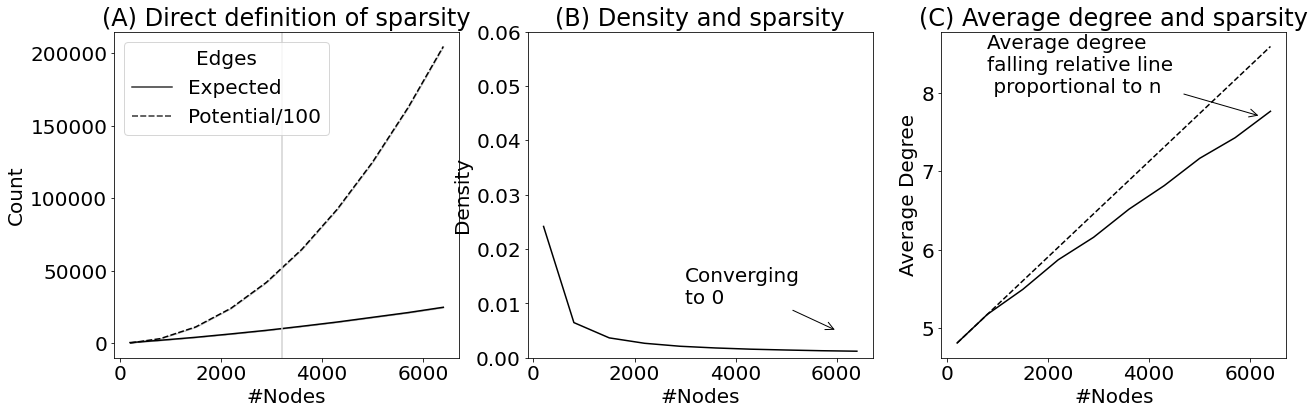
\includegraphics[width=\linewidth]{applications/ch7/Images/sparse_nets.png}
    \caption[Conceptualizing sparse networks]{\textbf{(A)} the direct definition of sparsity, \textbf{(B)} the equivalent definition of sparsity using the expected network density, \textbf{(C)} the equivalent definition of sparsity using the expected average node degree. Network sparsity has very specific definitions detailed in this section that must be proven out mathematically; illustrative plots like these are helpful to develop intuition for network sparsity, but are insufficient to prove that a sequence of random networks is sparse.}
    \label{fig:ch7:density:sparsity}
\end{figure}

\paragraph*{Relating sparsity to the network density}

Let's assume that we are given a value $\epsilon > 0$, and the $n_\epsilon$ such that the Equation \eqref{eqn:ch7:density:def1_condition} holds for all $n \geq n_\epsilon$.

Dividing through by $\binom n 2$ we see that for this $\epsilon$ and $n_\epsilon$ pair, that it is also the case that for all $n \geq n_\epsilon$:
\begin{align*}
    \mathbb E\left[density\left(\mathbf A^{(n)}\right)\right] &= \frac{\mathbb E\left[\sum_{j > i}\mathbf a_{ij}^{(n)}\right]}{\binom n 2} \leq \epsilon,\numberthis\label{eqn:ch7:sparse:density}
\end{align*}
where we simply used the definition of the expected density from Section \ref{sec:ch5:prop:rndens}. This shows that another equivalent characterization of sparse networks is that:
\begin{align*}
    \mathbb E\left[density\left(\mathbf A^{(n)}\right)\right] &= \smallO(1).
\end{align*}
or that, ``the expected density is decreasing to $0$ as the number of nodes grows''. 

We can repeat this with our experimental data by simply dividing the number of expected edges by the number of potential edges (adjusting for the normalization we made), like so:
\begin{lstlisting}[style=python]
df_wide = pd.pivot(df_mean.reset_index(), index="#Nodes", columns="Edges", values="Count")
df_wide["Density"] = df_wide["Expected"]/(100*df_wide["Potential/100"])
df_wide = df_wide.reset_index()
# plot it
sns.lineplot(data=df_wide, x="#Nodes", y="Density", color="black")
\end{lstlisting}

In the plot in Figure \ref{fig:ch7:density:sparsity}(B), we can see that for any choice of $\epsilon$, it looks like we could choose some value $n_\epsilon$ where the expected density is less than $\epsilon$.

\paragraph*{Relating sparsity to the expected average node degree}

Remember in Section \ref{sec:ch5:prop:rndens}, that we wrote the expected network density as:
\begin{align*}
    \mathbb E\left[density\left(\mathbf A^{(n)}\right)\right] &= \frac{\mathbb E[\mathbf d^{(n)}]}{n - 1},
\end{align*}
where $\mathbb E[\mathbf d^{(n)}] = \frac{1}{n}\sum_{i = 1}^n \mathbb E[\mathbf d_i^{(n)}]$ was the expected average node degree. 

Similarly, we can write that for the same choice of $\epsilon$ and $n_\epsilon$ as in Equation \eqref{eqn:ch7:sparse:density}, that if Equation \eqref{eqn:ch7:sparse:density} holds for any $\epsilon > 0$ and $n \geq n_\epsilon$, that it is also the case that:
\begin{align*}
    \mathbb E\left[density\left(\mathbf A^{(n)}\right)\right] = \frac{\mathbb E[\mathbf d^{(n)}]}{n - 1} &\leq \epsilon \\
    \Rightarrow \mathbb E[\mathbf d^{(n)}] &\leq (n - 1)\epsilon \leq n\epsilon,
\end{align*}
where the last inequality is because $\epsilon > 0$, so $(n - 1)\epsilon \leq n\epsilon$. This shows that in a sparse collection of networks, the expected node degree $\mathbb E\left[\mathbf d^{(n)}\right] = \smallO(n)$. 

This gives us our final equivalent characterization of sparse networks as networks where ``the expected average degree grows sublinearly with the number of nodes in the network''.

In the plot in Figure \ref{fig:ch7:density:sparsity}(C), we can see a diagonal line which grows with a rate proportional to $n$. Notice that the average node degree is growing slightly slower than the diagonal line (sublinearly).

\paragraph*{Equivalent characterizations of sparsity}
In total, we have three identical characterizations of \textit{sparse networks}:
\begin{enumerate}
    \item The expected number of edges grows slower than the number of potential edges: $\mathbb E\left[\sum_{j > i}\mathbf a_{ij}^{(n)}\right] = \smallO\left(\binom n 2\right)$,
    \item The expected network density is decreasing as the number of nodes grows: $\mathbb E\left[density\left(\mathbf A^{(n)}\right)\right] = \smallO(1)$, and
    \item The expected average degree grows slower than the number of nodes in the network: $\mathbb E[\mathbf d^{(n)}] = \smallO(n)$
\end{enumerate}
Note that all of these three definitions mean the exact same thing and are equivalent.

\begin{floatingbox}[h]\caption{Ultrasparse networks}
A further class of sparse networks, the \textit{ultrasparse} networks, is a collection of networks where $\mathbb E[\mathbf d^{(n)}]= \mathcal O(1)$. What this means is that ``the expected average degree is constant'', so the nodes in the network will have an average degree that does not grow as more nodes are added to the network. 

Note that the networks that we generate above do not appear to be ultrasparse, because the expected average node degree is growing (albeit, slower than the number of nodes is increasing). To determine whether it is leveling off to a constant, or just leveling off (but still growing to infinity as $n \rightarrow \infty$) would take a background in real analysis.
\end{floatingbox}

\subsection{Data wrangling and matrix sparsity}

In addition to network sparsity a substantial nuisance when running many standard network learning techniques, matrix sparsity plays a big role in the data wrangling step for network data. \textit{Data wrangling} refers to the process of manipulating data (your network) into a format that makes it more appropriate and valuable for your analytical purposes. An $n \times d$ matrix with non-negative entries is said to be \textit{sparse} if any of its entries are zero. On the other hand, an $n \times d$ matrix with non-negative entries is said to be \textit{dense} if none of its entries are zero.

We further subset these to say that a matrix is \textit{sufficiently sparse} if the matrix has enough of a fraction of the entries being zero that it makes sense to take advantage of it.

Let's take a look at some applications of matrix sparsity. Our working example will be a sample of our academic networks above, with $K = 10$ communities and $n=1000$ nodes:

\begin{lstlisting}[style=python]
A, zs, P = academic_example(10)

print("# Non-zero entries: {:d}".format(np.triu(A).sum().astype(int)))
# Non-zero entries: 3163
print("# Number of entries: {:d}".format(np.triu(np.ones((n, n))).sum().astype(int)))
# Number of entries: 20483200
\end{lstlisting}

A plot of the network adjacency matrix is shown in Figure \ref{fig:ch7:density:deg}(C).

\paragraph*{Storage implications of sparse adjacency matrices with network data}

Throughout this book, we have typically encountered networks as dense adjacency matrices. This means that we stored the entire adjacency matrix (all $n \times n$ entries). When the adjacency matrix is sufficiently sparse, this can be an extremely inefficient approach to handling network data. 

The network above has $n=1000$ nodes. The most naive way to store the adjacency matrix, which we do frequently in this book, is to store it as a $n \times n$ matrix, which means that we have $1000000$ entries. Each of these entries defaults to a \texttt{float64} in numpy, which is a $64$-bit number. This means that our network, in total, occupies $1000^2 \cdot 64 = 64$ million bits (Mb), or $64/8 = 8$ million bytes (MB). 

However, we have a lot of redundancies here. First, the network is simple, so edges are unweighted. When the edges are unweighted, we only need a single bit to represent each number. Unfortunately, RAM on your computer is divided by bytes, so the best we could do is $1$ byte per entry using standard \texttt{python} approaches. We will cast each entry of \texttt{A} to a \texttt{uint8}, which is an $8$ bit unsigned integer. That it is unsigned simply means that the entry cannot be negative. Let's see how much space we save:

\begin{lstlisting}[style=python]
# before conversion
print("Size in KB: {:3f} KB".format(A.nbytes/1000))
# Size in KB: 8000.000000 KB

B = A.astype(np.uint8)
print("Size in KB: {:3f} KB".format(B.nbytes/1000))
# Size in KB: 1000.000000 KB
\end{lstlisting}

The byte separation issue aside, this is still considerably more space than necessary. First, the total number of entries being stored is $1000^2 = 1$ million, but there are only $\binom n 2 = .4995$ million unique entries (remember that a simple network is loopless and undirected, which means that we only need to keep track of the upper triangle of the adjacency matrix, and we can ignore the diagonal entries entirely) so we are overcounting by about a factor of two. 

This means that we could simply ignore everything but the upper triangle, and still ``recover'' the entire adjacency matrix. Let's see how to do this with \texttt{scipy} sparse matrices:

\begin{lstlisting}[style=python]
import scipy.sparse as sparse

Btriu = sparse.triu(B)
print("Size in KB: {:3f}".format(Btriu.data.size/1000))
# Size in KB: 3.163000
\end{lstlisting}

So this has reduced the size of the network from $8000$ KB to just $3.066$ KB, which is about three hundred times smaller.

So, how did \texttt{scipy} do this for us?

Let's just print out \texttt{Btriu} and see what \texttt{scipy} did:

\begin{lstlisting}[style=python]
Btriu
# <1000x1000 sparse matrix of type '<class 'numpy.uint8'>'
#   with 3163 stored elements in COOrdinate format>
\end{lstlisting}

\texttt{COOrdinate} format is an extremely efficient way to represent the entries of a sparse adjacency matrix. To illustrate the \texttt{COOrdinate} format, let's imagine that we have the simple $5 \times 5$ adjacency matrix for a network with $5$ nodes shown below:
\begin{align*}
    A &= \begin{bmatrix}
        0 & 1 & 0 & 1 \\
        1 & 0 & 0 & 0 \\
        0 & 0 & 0 & 1 \\
        1 & 0 & 1 & 0
    \end{bmatrix}\numberthis \label{eqn:ch7:sparsity:adjex}
\end{align*}

Basically, what \texttt{scipy} does is it stores the matrix like is shown in Table \ref{tab:coordfmt}. It looks at each non-zero edge in the upper triangle of the adjacency matrix for the network (for instance, $a_{12} = 1$, so we will arbitrarily call this the first edge), and then records the row and column of those edges. The second edge is $a_{14} = 1$, and the third edge is $a_{23} = 1$. The adjacencies in the lower triangle ($a_{21}$, $a_{41}$, and $a_{32}$) are redundant, so they are omitted from this representation entirely.

\begin{table}[h]
    \centering
    \begin{tabular}{c|c| c}
        Row & Column & Value \\
        \hline
         1 & 2 & 1\\
         1 & 4 &  1 \\
         2 & 3 &  1
    \end{tabular}
    \caption[\texttt{COOrdinate format} for sparse matrices]{The adjacency matrix in Equation \eqref{eqn:ch7:sparsity:adjex}, in \texttt{COOrdinate} format. For larger networks, this pattern would continue for every non-zero entry in the adjacency matrix.}
    \label{tab:coordfmt}
\end{table}

So, in effect, \texttt{scipy} completely ignored storing the matrix entry-wise all-together: it simply stored the rows and columns of the upper-triangular non-zero entries of \texttt{B}, each as a single byte. Next, it stored the total size of the matrix in another spot (which was $1000 \times 1000$) so that you can ``recover'' the entire matrix \texttt{B} from the \texttt{COOrdinate} format in \texttt{Btriu}. Remember that since the underlying network was simple, you can just use utilities to symmetrize \texttt{Btriu} that we developed in Section \ref{sec:ch4:regularization:symmetrize} if you want to recover the original matrix \texttt{A}.

\begin{lstlisting}[style=python]
from graspologic.utils import symmetrize

# cast the sparse matrix back to a dense matrix,
# and then triu symmetrize with graspologic
A_new = symmetrize(Btriu.todense(), method="triu")
np.alltrue(A_new == A)
# True
\end{lstlisting}
If you have sufficiently sparse adjacency matrices, you can exploit this structure just like we have here to get vastly improved spatial performance storing your networks. Since really sizable networks tend to be sufficiently sparse, the most common storage format you will find with simple networks is something similar to this \texttt{COOrdinate} format, called an edge list, which is a \texttt{csv} (comma-separated values), \texttt{ssv} (space-separated values), or \texttt{tsv} (tab-separated values) file, like is shown in Table \ref{tab:adjlist} for the simple example in Equation \eqref{eqn:ch7:sparsity:adjex}. With \texttt{csv} or \texttt{ssv} formats, instead of having tabs separate the node indexing columns of the edge list, you could also have spaces or commas (or any suitable delimiter). 

\begin{table}[h]
    \centering
    \begin{tabular}{c| c}
        Node $1$ & Node $2$  \\
        \hline
         1 & 2\\
         1 & 4 \\
         2 & 3
    \end{tabular}
    \caption[Edgelist network storage format]{The upper triangle of the adjacency matrix, stored as a \texttt{tsv} (tab-separated values) file, for the adjacency matrix in Equation \eqref{eqn:ch7:sparsity:adjex}.}
    \label{tab:adjlist}
\end{table}

Depending on the classification of the network that you are working with, the appropriate format for storage might differ. When networks are simple, the strategy described above (an edgelist, where each line indicates the node indices of non-zero entries in the upper triangle of the adjacency matrix) tends to be a format you will commonly come across. When the network is weighted, there is often a third column corresponding to the edge-weight, which is redundant in unweighted networks (and therefore often omitted entirely). When the network is directed, the lower triangle entries are also typically stored. When the network is undirected but includes loops, the edgelist will typically include the all nodes in the upper triangle, in addition to the diagonal. 

With so many possible representations of networks in edgelist or sparse formats, it is imperative when you work with real networks that you first ascertain the underlying properties of the network that you are working with. Understanding the properties of the underlying network will indicate to you how to properly ``unpack'' an edgelist or sparse representation to recover an adjacency matrix.

\paragraph*{Algorithmic implications of matrix sparsity}

When you represent the adjacency matrix using sparse formats, you can benefit a lot by leveraging algorithms designed for sparse data. Let's see, for instance, how long it takes for \texttt{scipy} to run a sparse \texttt{svd} when we pass the data in a dense format (a standard \texttt{numpy} array) and use a standard \texttt{svd}, compared to when we use a sparse format and use a partial \texttt{svd}, to embed into $20$ dimensions. A full \texttt{svd} for an $n \times n$ square matrix (remember that adjacency matrices are square) will compute all $n$ left and right singular vectors (along with their singular values). A partial \texttt{svd} will only compute the top (or bottom) subset of these:

\begin{lstlisting}[style=python]
import time

# a naive full svd on the dense matrix
timestart = time.time()
U, S, Vh = sp.linalg.svd(A)
Xhat = U[:, 0:20] @ np.diag(np.sqrt(S[0:20]))
timeend = time.time()
print("Naive approach: {:3f}".format(timeend - timestart))
# we get about .35 seconds

# a sparse svd on the sparse matrix
Acoo = sparse.coo_array(A)
timestart = time.time()
U, S, Vh = sp.sparse.linalg.svds(Acoo, k=20)
Xhat = U @ np.diag(np.sqrt(S))
timeend = time.time()
print("Sparse approach: {:3f}".format(timeend - timestart))
# we get about .08 seconds
\end{lstlisting}

Which is about a factor of four improvement in speed. As matrices grow in size, and have a lower and lower fraction of their entries being non-zero, sparse approaches tend to dramatically outperform naive implementations. 

At a certain point, when your data gets really large, you might not even be able to execute standard functions on standard arrays, and might be required to use sparse approaches.

\subsection{Practical applications of network sparsity and matrix sparsity}

Matrix and network sparsity have a unique interplay when dealing with network data represented as an adjacency matrix. This case we will consider deals directly with a strategy that you have gotten quite accustomed to at this point in the book: spectral embeddings of network data. For this example, we will see a unique problem that the adjacency spectral embedding can run into with sparse networks that have sparse adjacency matrices.

Let's consider our example from the above section with $K=10$ communities and $n=1000$ nodes. The underlying probability matrix and the adjacency matrix for the network are shown in Figure \ref{fig:ch7:density:deg}(A) and (B) respectively. We can see some fairly prominent modular structure, so from what we learned in Chapter \ref{ch6} and Section \ref{sec:ch7:comm_detect}, a reasonable approach to learn from the data might be a spectral embedding and a clustering to identify community assignments from the network. To determine whether \texttt{lse} or \texttt{ase} are appropriate for our data, we compute the node degrees like we did for Section \ref{sec:ch6:lse}:

\begin{lstlisting}[style=python]
degrees = A.sum(axis=0)
\end{lstlisting}

The degree distribution for the network is shown in \ref{fig:ch7:density:deg}(C). The degree distribution looks extremely right-skewed/heavy-tailed, so from Section \ref{sec:ch6:lse}, an appropriate choice would be to do a spectral embedding with \texttt{lse}.

\begin{figure}[h]
    \centering
    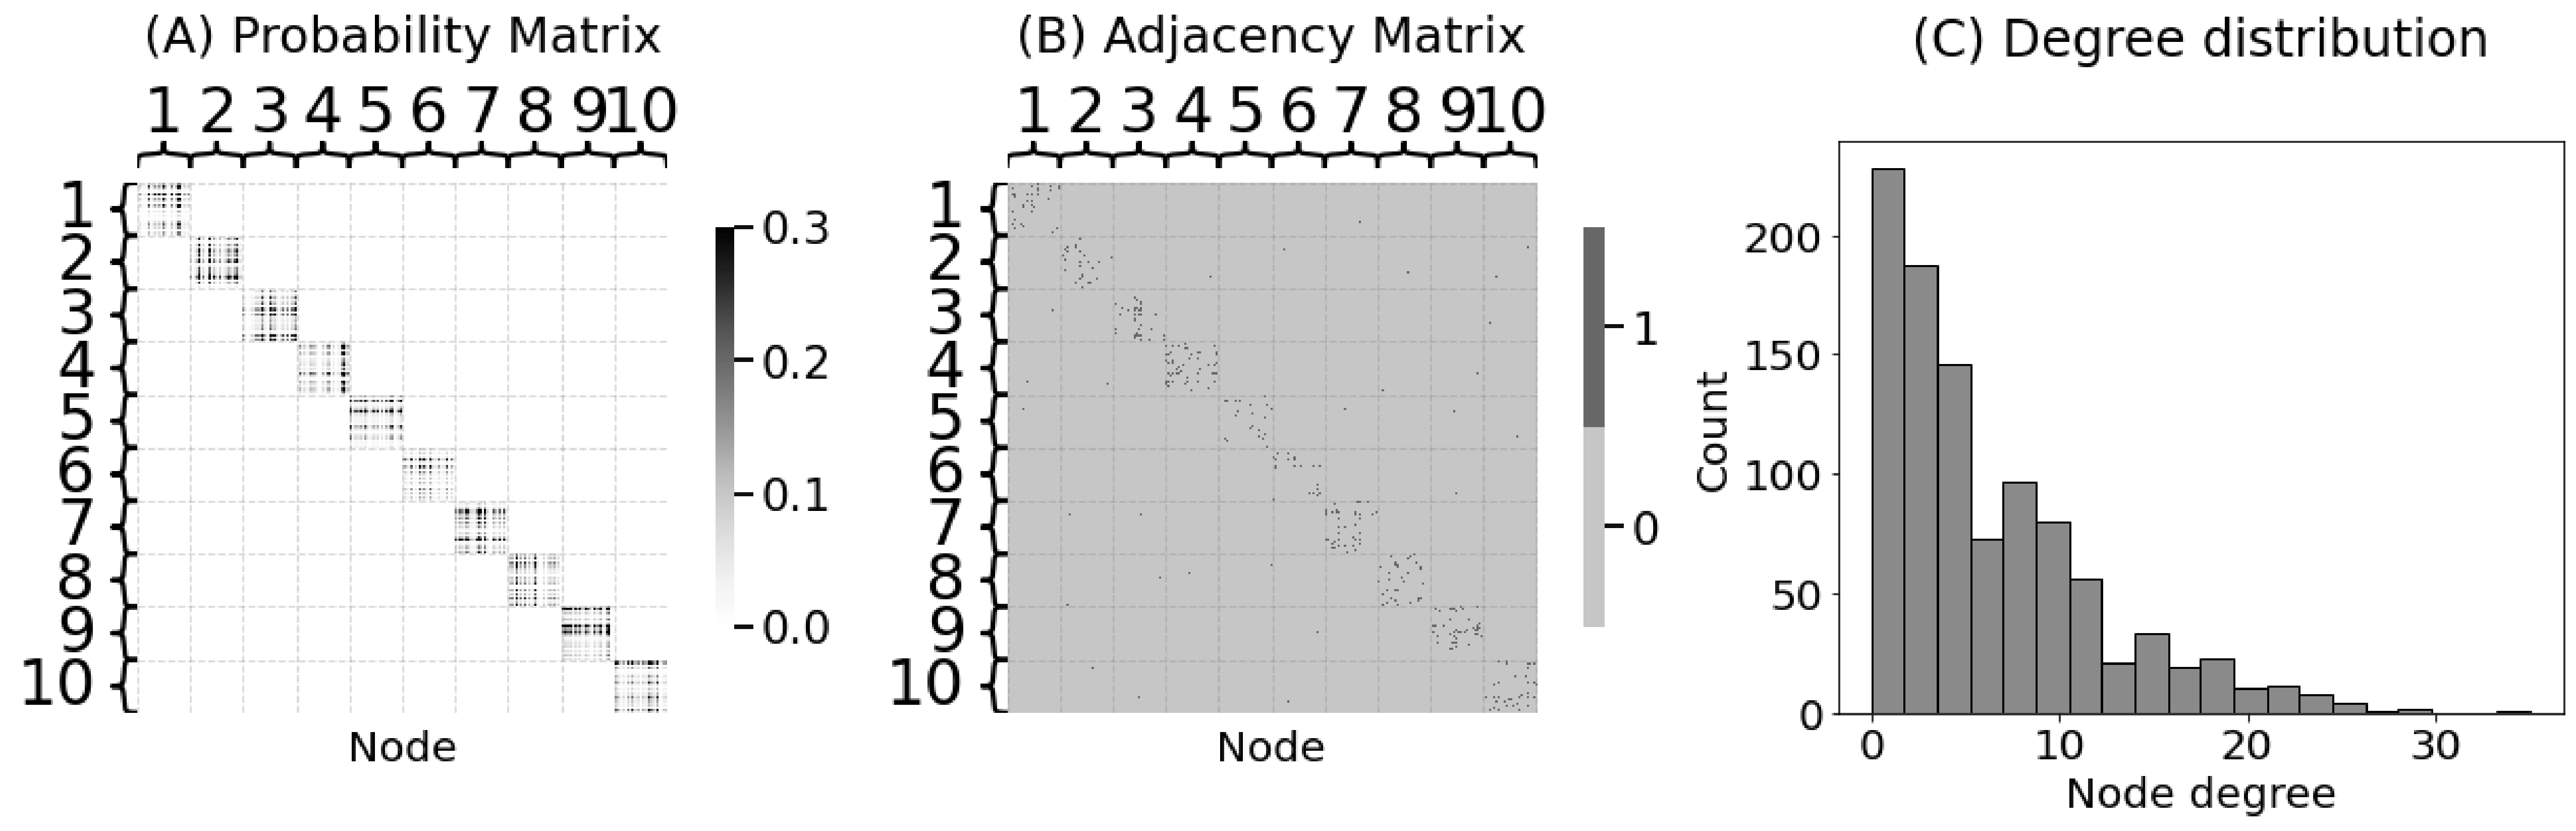
\includegraphics[width=\linewidth]{applications/ch7/Images/eigenspoke_ex.png}
    \caption[Network sample from sparse networks]{\textbf{(A)} the probability matrix, \textbf{(B)} the adjacency matrix, and \textbf{(C)} the heavy-tailed degree histogram for a network from a sparse sequence of networks.}
    \label{fig:ch7:density:deg}
\end{figure}

To do this, we're going to look at the top $5$ left singular vectors of the \texttt{DAD} Laplacian, remembering that \texttt{lse} is a function of these vectors (rescaled by the eigenvalues) in Algorithm \ref{alg:ch6:lse}. We will do this with \texttt{scipy}'s sparse \texttt{svd}, which we learned above is much faster for sparse data than a full \texttt{svd} with numpy:

\begin{lstlisting}[style=python]
import scipy as sp
from graspologic.utils import to_laplacian
from graspologic.plot import pairplot

# use sparse svd, so that we don't need to compute
# 1000 singular vectors and can just calculate the top 5
U, S, Vh = sp.sparse.linalg.svds(to_laplacian(A), k=5)
pairplot(U, labels=zs, title="Eigenspokes in the Laplacian")
\end{lstlisting}

We visualize the top $4$ singular vectors as a pairplot in Figure \ref{fig:ch7:density:pair}(A). Remember that each node is a point in this plot. What we notice is rather unusual. In many dimensions, such as dimensions $1$ and $2$ in particular, nodes appear to basically have an ``all or nothing'' pattern: entire communities of nodes have a $0$ for along almost all of the singular vectors, except for the long spoke that they stretch along. For instance, in dimension $2$, notice that the red community occupies the bottom of the dimension, and a combination of the pink, green, and blue communities occupy the top of the dimension. Likewise, along dimension $1$, we can see that the green community occupies the entire top of the dimension, and the yellow community occupies the entire bottom of the dimension. Along many of the other dimensions, such as $3$ and $4$, almost all of the nodes simply have a value of $0$. 

This ``all-or-nothing'' pattern is what is known as an \textit{EigenSpoke} \cite{Prakash2010}: some communities are clearly separated along axes, but have no separation along other axes. This all-or-nothing EigenSpoke behavior presents an extreme challenge for techniques like \texttt{KMeans} and \texttt{GMM}, which tend to favor spherical and elliptical ``blobs'' respectively.

\begin{figure}[h]
    \centering
    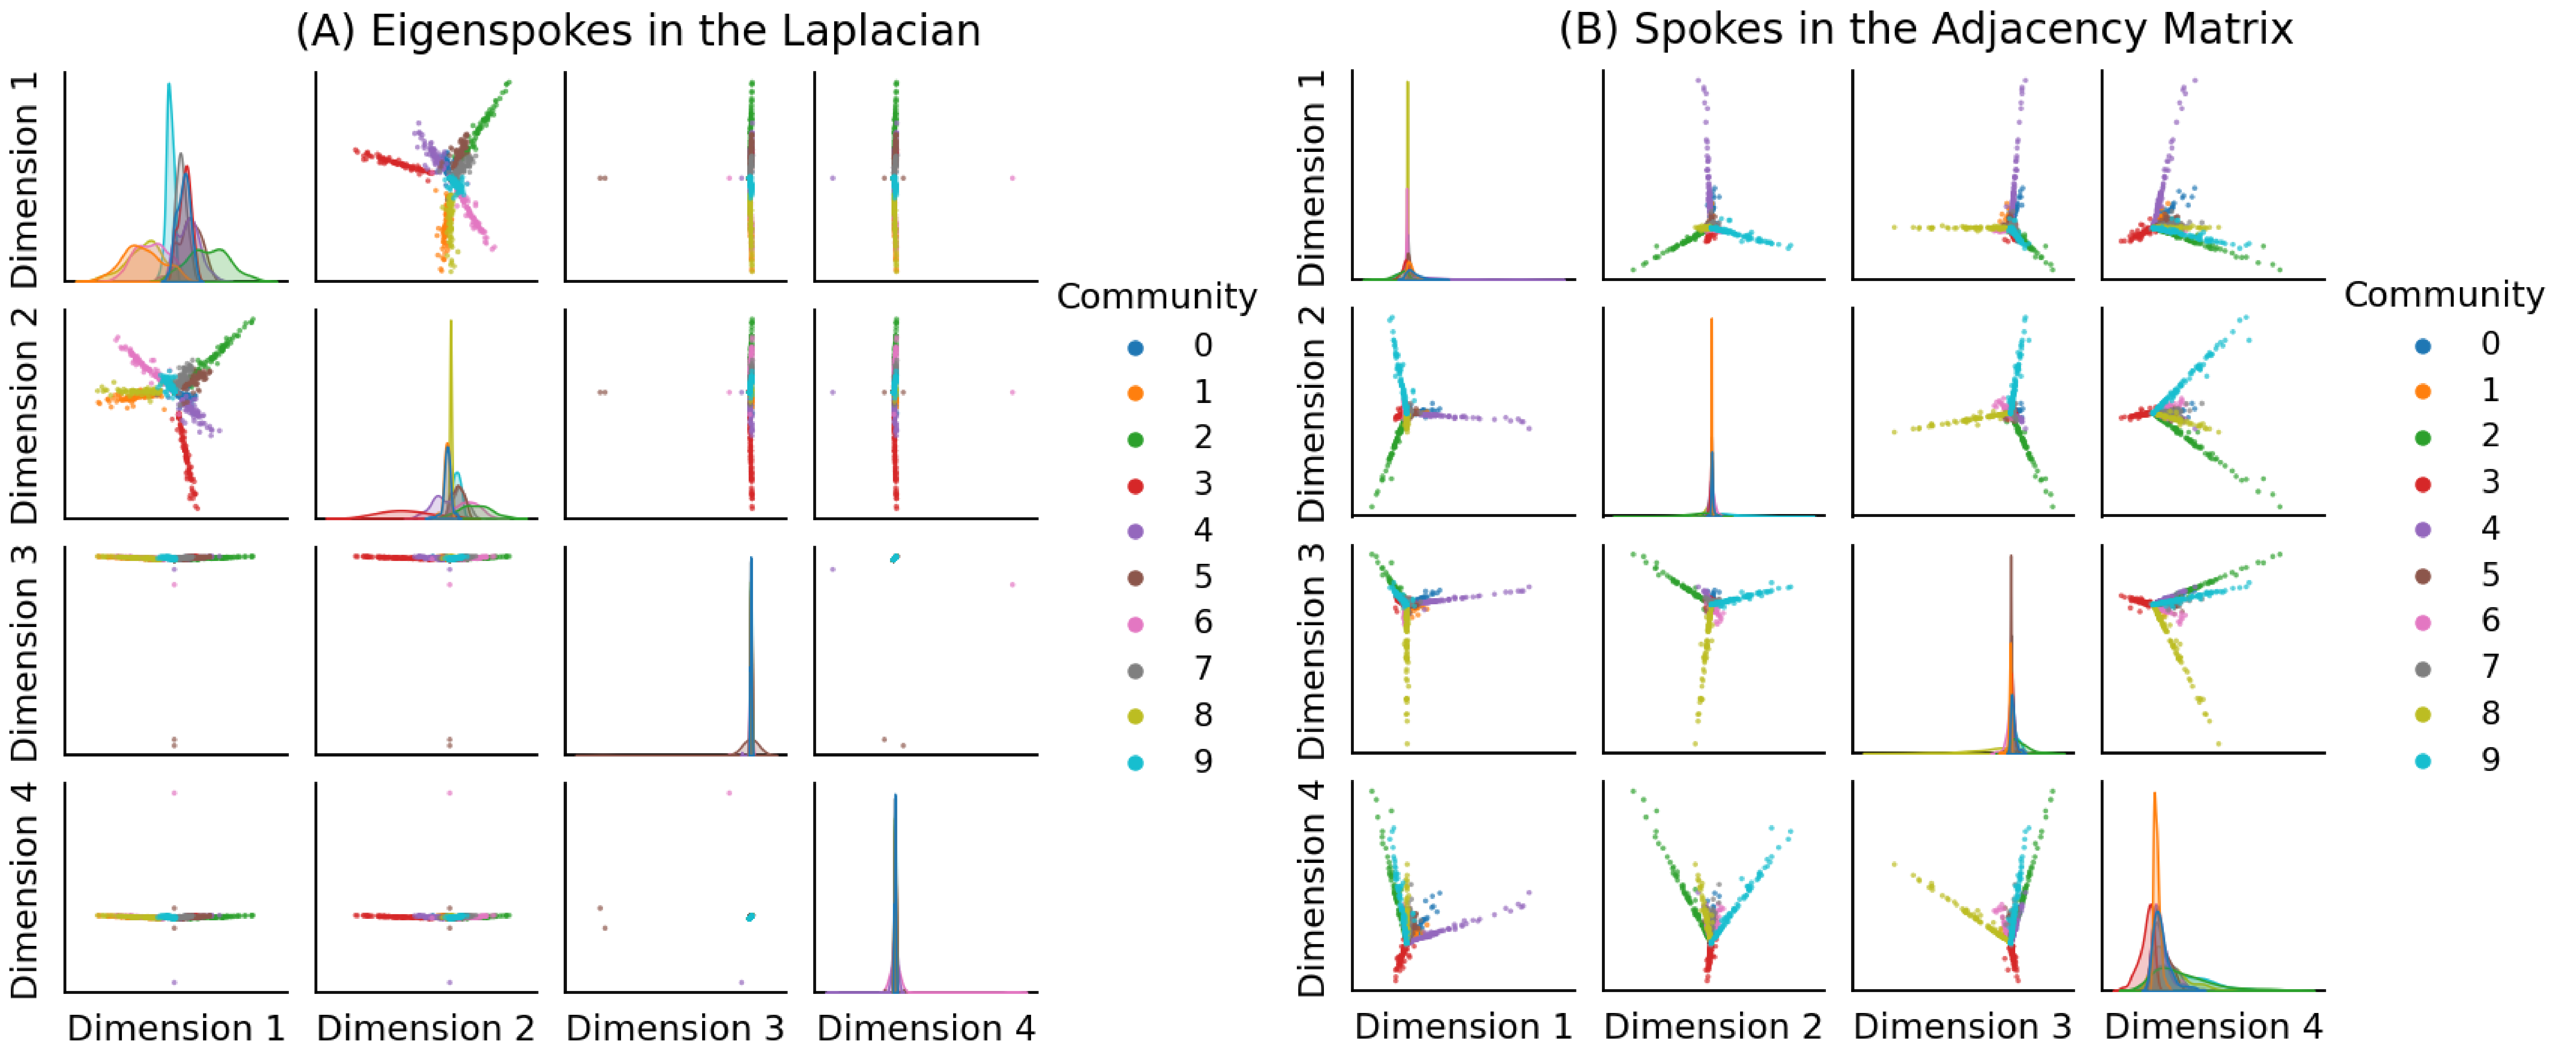
\includegraphics[width=\linewidth]{applications/ch7/Images/eigenspokes.png}
    \caption[Spokes in spectral embeddings of sparse adjacency matrices]{\textbf{(A)} Eigenspokes in the singular vectors of the laplacian, \textbf{(B)} moderate spokes in the singular vectors of the adjacency matrix.}
    \label{fig:ch7:density:pair}
\end{figure}

It seems pretty clear from the intuition that we gained in Section \ref{sec:ch7:comm_detect} that we don't appear to have the setup that \texttt{KMeans} or \texttt{GMM} do well in (structured blobs in the pairplots), so let's try looking at the singular vectors associated with the \texttt{ase} instead of the \texttt{lse}:

\begin{lstlisting}[style=python]
U, S, Vh = sp.sparse.linalg.svds(A, k=5)
pairplot(U, labels=zs, title="Eigenspokes in the Laplacian")
\end{lstlisting}

These aren't quite ``EigenSpokes'', in that the points aren't perfectly axis-aligned, but they're still quite spokey in shape. Here, too, naive community detection approaches will struggle, even though some of the communities look less poorly separated. To convince yourself as to why community detection with \texttt{kmeans} might fail, we would encourage you to visualize the distance matrix between pairs of nodes, like you did in Section \ref{sec:ch6:lse}, armed with the intuition that you gained in Section \ref{sec:ch7:comm_detect} about \texttt{kmeans} for community detection.

As it turns out, spectral approaches tend to struggle with networks that can be thought of as sparse (which, as we saw in Figure \ref{fig:ch7:density:sparsity}, it is). You can identify when you might run into these patterns by looking at how sparse the adjacency matrix is. You will typically run into sparse network troubles when the number of edges is ``on the order of'' the number of nodes in the network, and when it is far less than the number of potential edges in the network. You can calculate these with:

\begin{lstlisting}[style=python]
print("# Expected edges: {:2f}".format(np.triu(P).sum()))
print("# True edges: {:d}".format(np.triu(A).sum().astype(int)))
print("# Potential edges: {:d}".format(np.triu(np.ones((n, n))).sum().astype(int)))
# Expected edges: 3208.041454
# True edges: 3060
# Potential edges: 500500
\end{lstlisting}

When you run into situations where the number of edges is orders of magnitude less than the number of potential edges, you should be on the lookout for potentially running into sparsity concerns and be aware that many naive spectral techniques (such as \texttt{ase}, \texttt{lse}, and derived approaches like \texttt{mase} and \texttt{omni}) will struggle to produce embeddings that will facilitate downstream analysis (like community detection) \cite{Lei2013Dec}. You may need to turn to alternative techniques such as \cite{Krzakala2013Dec,Chen2012} to achieve high performance in these settings, where you incorporate different functions of the adjacency matrix that are better behaved for sparse regimes all together or apply penalties to nodes with low degrees to, in some sense, force your embeddings to avoid these spoke-like patterns.

\begin{floatingbox}[h]\caption{Simulating EigenSpokes is not an exact science}
EigenSpokes are a phenomena that arise in sparse networks, in that we have a good idea of what situations they can arise in (sparse networks) but not a great idea of how to reliably obtain them from random network samples. 

In this sense, you may have to run your simulations a few times to produce perfect ``EigenSpoke''-like patterns that run perfectly parallel along eigenvectors. They shouldn't be too hard to come by; when running these examples listed here, I tended to get spokes about $50\%$ of the time (and nonsensical embeddings in the other cases). 
\end{floatingbox}

\paragraph*{What does network sparsity have to do with these phenomena we observed with sparse adjacency matrices?}

The way that network sparsity fits into these strategies is a little bit indirect. First, we defined sparsity as a property that occurs over a sequence of random networks, which does not quite fit into real networks. Next, we showed that when a network had relatively few entries (its adjacency matrix was sparse), we could identify odd behaviors in particular algorithms, like the \texttt{lse} and \texttt{ase}. These two ideas feel at odds because the definition of sparsity does not apply to network samples, but in practice, we only have network samples.

Remember in Section \ref{sec:ch6:ase:whyuse}, we justified the \texttt{ase} by arguing that, when we have a network sample from a random network, as the network gets larger and larger, the estimated latent position matrix gets closer and closer to the true latent position matrix of the underlying random network. However, there is a caveat attached to this result: the underlying random network must have a probability matrix that obeys certain conditions \cite{Athreya2017Jan,Krzakala2013Dec} that ensure that the sequence of networks are not sparse. 

These conditions go a bit beyond the scope of this book, but the idea is that when the networks fail to satisfy these regimes, the naive \texttt{ase} loses its meaning. As the number of nodes increases, instead of the estimated latent position matrices getting closer and closer to the true latent position matrix of the underlying random network, the estimates become progressively more nonsensical. At some level, we lose the ability to say that $\hat X$ (the estimated latent position matrix) is a reasonable estimate of the true underlying latent position matrix $X$. This is why we observed ``puzzling'' behaviors in the spectral embeddings of our networks here (which were samples from a sparse sequence of random networks). 

\begin{floatingbox}[h]\caption{Complementary definitions of sparsity}
These two definitions of sparsity differ in that \textit{network sparsity} is a property of an underlying sequence of random networks, but \textit{matrix sparsity} is a property of the adjacency matrix (or a function thereof) for a network that you obtain. 

A network with a sufficiently sparse adjacency matrix will often run into problems associated with sparse sequences of random networks, and samples from sparse sequences of networks with enough nodes will often have sufficiently sparse adjacency matrices to cause odd results in network learning algorithms, so these two definitions prove complementary in network science.
\end{floatingbox}

\newpage
\section{Testing for differences between groups of edges}
\label{sec:ch7:testing}

Over the last few sections, we have covered a lot of information about stochastic block models and degree-corrected stochastic block models. As you learned in Section \ref{sec:ch5:siem}, the stochastic block model can be generalized to the Structured Independent Edge Model, or SIEM, in that all $SBM_n(\vec z, B)$ random networks could be reformulated as a $SIEM_n(C, \vec p)$ random network. 

The parameter $C$ defined individual ``clusters'' of edges in the network, where entry $c_{ij}$ indicated which edge cluster (of $K$ total edge clusters) the edge between nodes $i$ and $j$ were assigned. The probability vector $\vec p$ had $K$ elements, where the entry $p_k$ indicated the probability of an edge for edges which were assigned to cluster $k$.

When you have a network, if you have a set of node or edge groupings, you can therefore conceptualize your network as a sample of a $SIEM_n(C, \vec p)$ random network. You learned in Section \ref{sec:ch6:mle} how to estimate probabilities from collections of edges, and these strategies apply readily to the $SIEM_n(C, \vec p)$ random networks as well. 

By the same argument as we made in that section, if you have a network sample with edge clusters given by the matrix $C$, you could compute the estimated probability for edges in cluster $k$ with:
\begin{align*}
    \hat p_k &= \frac{\sum_{i, j : c_{ij} = k}a_{ij}}{n_k},
\end{align*}
where $n_k$ is the total number of edges which are assigned to cluster $k$, and is given by $\sum_{i, j : c_{ij} = k}1$. The sums here are over all possible edges, but excludes to only look at edges where the edge is assigned to cluster $k$.

To make this example a little more concrete, let's return to our $SIEM_n(D, \vec p)$ example from Section \ref{sec:ch5:siem}, and use a probability vector $\vec p^\top = [0.3, 0.7]$. We can build the edge cluster assignment matrix and a probability vector like this:

\begin{lstlisting}[style=python]
import numpy as np
from graphbook_code import siem

n = 100
D = np.ones((n, n))
for i in range(0, int(n/2)):
    D[int(i + n/2), i] = 2
    D[i, int(i + n/2)] = 2
np.fill_diagonal(D, 0)

p = [0.4, 0.6]
A = siem(n, p, D)
\end{lstlisting}

\begin{figure}
    \centering
    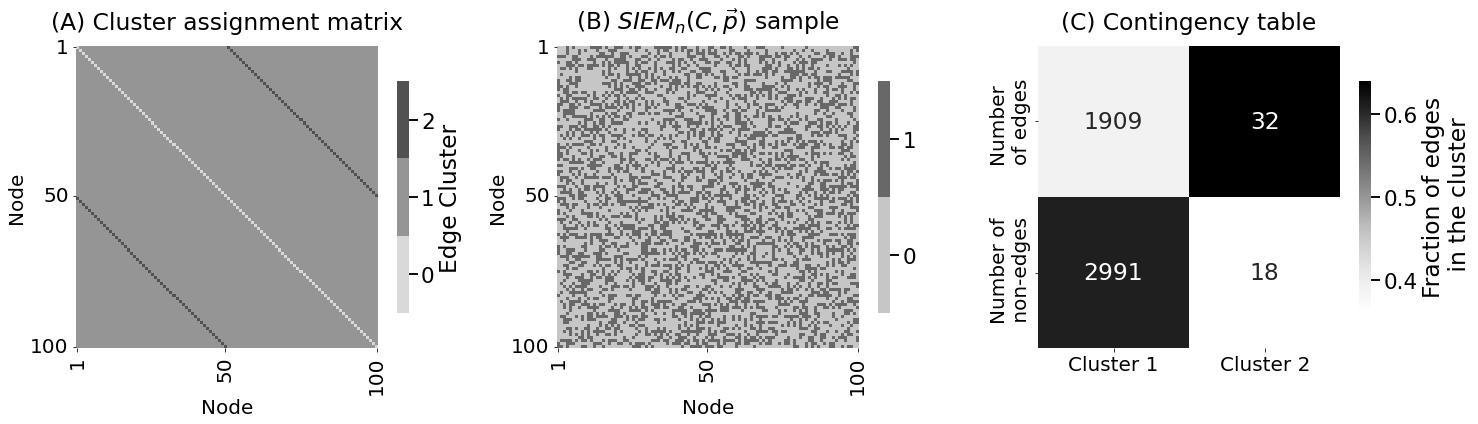
\includegraphics[width=\linewidth]{applications/ch7/Images/testing_siem_ex.png}
    \caption{\textbf{(A)} the edge-cluster assignment matrix, \textbf{(B)} the adjacency matrix, \textbf{(C)} a contingency table for the two edge-clusters in the network sample.}
    \label{fig:ch7:testing:siem_ex}
\end{figure}
The edge cluster assignment matrix $C$ is shown in Figure \ref{fig:ch7:testing:siem_ex}(A), and a sample of the network is shown in Figure \ref{fig:ch7:testing:siem_ex}(B). When we look at the network in Figure \ref{fig:ch7:testing:siem_ex}(B), the edges corresponding to edge-cluster $2$ in Figure \ref{fig:ch7:testing:siem_ex}(A) look to stand out a little bit from the other edges, but it looks far from definitive at a glance. We can compute the estimated edge probabilities (per edge-cluster) using the below code:

\begin{lstlisting}[style=python]
est_pvec = []
for k in [1, 2]:
    # compute the estimated pvalue for cluster k as the 
    # fraction of non-zero entries, which is the sample mean
    est_pvec = A[D == k].mean()
print(est_pvec)
# [0.3895918367346939, 0.64]
\end{lstlisting}
So the estimated edge probabilities appear to be quite different just looking at the sample. When we observe the sample, we don't at first glance know that the underlying random network truly has a different probability for each edge cluster. We only see the network sample, which will never perfectly reflect the underlying random network model that we think is appropriate for the sample. This means that if we want to determine whether the estimated edge probabilities are appreciably different, we have some work to do.

\subsection{Two-sample hypothesis testing}

As explained in Remark \ref{box:ch7:testing:twosample_coin}, when you have two samples of data, a key question you may have as a scientist is determining whether the nuances you observe in the sample are down to random chance, or whether the difference is substantial enough that the two samples might actually have fundamental differences. This is known as a \textit{two-sample test}.

\begin{floatingbox}[h]\caption{The problem of reading too much into estimates}
\label{box:ch7:testing:twosample_coin}
Let's imagine that your friend comes to you with a game. They gives you a coin, and he has a coin for himself. They assert that whomever has the coin that lands on heads most wins, and receives the title of ``masterful coin flipper'' for all of eternity. You each perform your coin flips, and you get four heads and your friend gets six heads. In this case, we have two samples of data: the outcomes of the coin flips for each of your coins. 

From what we learned in Section \ref{sec:ch6:mle}, if you wanted to estimate the probability that each of your coins land on heads, a reasonable approach would be to sum up the number of heads, and divide by the total number of coin flips. Using this strategy (the maximum likelihood estimate), you would arrive at an estimate of $\frac{4}{10}$ for the coin that you flipped, and $\frac{6}{10}$ for the coin your friend flipped.

Next, you decide to ask a question: what are the chances that your friend rigged this game in some way? What are the chances that the coins we used were fundamentally different, and that the underlying probabilities that each coin which we flipped were different? 

Indeed, it is the case that even a fair coin will not always produce exactly half of the coin flips as heads when you flip it $n$ times (just try flipping a coin nine times and see whether you get four and a half outcomes of heads!). Even if you flip the coin an even number of times, you're still probably not going to get exactly $\frac{n}{2}$ heads. Try flipping a coin ten times, and repeat it a few times, and count how many of your ``trials'' produce exactly five heads. 

Before you go to your friend and accuse them outright of cheating, you would probably want to know what the chances are that your coin (if they were fair) would have produced the disparate estimates of $\frac{4}{10}$ as compared to $\frac{6}{10}$. Stated another way, you want to be able to determine whether the two samples of data that you have are fundamentally different, or if the difference is just dumb luck.
\end{floatingbox}

To rotate back to the $SIEM_n(C, \vec p)$ random network example, a sample of our network $A$ has edges $a_{ij}$ which are binary valued. What we want to do is test for a pair of communities $k$ and $l$ (which are two of the $K$ total clusters in our network), we want to choose between a pair of ways to describe our system. These options are known as \textit{hypotheses} for a hypothesis test. In this case our hypotheses are:
\begin{align*}
    H_0 : p_k = p_l \text{ against }H_A : p_k \neq p_l
\end{align*}
The \textit{null hypothesis} is the hypothesis where, if true, indicates that we were wrong about how we thought that the system behaved. In our example, our null hypothesis is that $p_k = p_l$, or that the underlying probabilities are identical between the two clusters. The capital $H$ denotes that this is a hypothesis, and the lowercase $0$ just indicates ``null''.

The \textit{alternative hypothesis} is the hypothesis where, if true, indicates that we are correct about how we think the system behaves. In our example, the alternative hypothesis is that $p_k \neq p_l$, or that the underlying probabilities differ between the two edge-clusters. 

When we read the hypothesis, we read it is: we are testing $H_0$ the null that $p_k = p_l$ and the underlying probabilities are identical against $H_A$ the alternative that $p_k \neq p_l$ and the underlying probabilities differ. The reason that our hypothesis is structured in this way is that the hypothesis test must delineate the possible situations in which we are right (the alternative) and we are wrong (the null). 

Using hypothesis tests to learn about an underlying system is a component of what is known as \textit{statistical inference}, or using statistics to make informed decisions about how a system behaves. We perform statistical inference with hypothesis tests by looking at how well the data that we are presented with reflect the null hypothesis. This means that either the data looks like what we would expect under the null hypothesis, or the data does not look like what we would expect under the null hypothesis. We convey the degree to which the data looks different from what we would expect under the null hypothesis with the $p$-value, which is explained in Remark \ref{box:ch7:testing:pval}.

\begin{floatingbox}[h]\caption{The $p$-value is the unit used for decision making in hypothesis tests}
\label{box:ch7:testing:pval}
When performing hypothesis tests, the fundamental unit that is used for decision making is known as a $p$-value. The $p$-value is:
\begin{align*}
    p &= Pr\left(\text{ we falsely reject $H_0$ in favor of $H_A$} \big| H_0\text{ is true}\right)
\end{align*}
The vertical bar in statistics means ``conditioned on'', which means that the probability is being computed with the assumption that the null hypothesis is true. The implications of this statement are critical to a quality statistical analysis, so let's break it down.

For a hypothesis test, we first begin by deciding the assumptions that we have about how the system behaves. For network science, these assumptions are conveyed by the statistical models that you learned in Chapter \ref{sec:ch5}.

After you assume the statistical model, your hypotheses will typically reflect facts about how the data behaves with respect to the parameters that you chose. For instance, in the $SIEM_n(D, \vec p)$ model, you assume that the edges $\mathbf a_{ij}$ are independent coin flips with probability given by $p_{d_{ij}}$. 

Finally, the way that we structure the null hypothesis is usually lined up with something that we know the distribution of. In the example of coin flips in Remark \ref{box:ch7:testing:twosample_coin}, we can explicitly determine the amount of variation that we would expect in the number of heads that two identical coins would receive in a particular number of coin flips. 

Intuitively, using the actual number of heads from our two smples, we can then assert whether the actual number of heads that we obtain is ``close enough'' to the level of variability that we would have expected, or whether it is vastly different than what we would have expected if the two coins were the same. 
\end{floatingbox}

\subsection{Two-sample hypothesis testing with binary-valued data}

Let's rotate to the coin flip example. In this case, our hypothesis is that:
\begin{align*}
    H_0 : p_1 = p_2 \text{ against }H_A : p_1 \neq p_2. \numberthis \label{eqn:ch7:testing:hypo_coin}
\end{align*}
When each of the two samples (the ten coin flips from each of the two coins) are independent and have binary-valued outcomes (heads or tails), a common summary measure is known as a contingency table. The contingency table is shown in Table \ref{tab:ch7:testing:cont}.

\begin{table}[h]
    \centering
    \begin{tabular}{c | c|c}
         & Your coin & Your friend's coin  \\
         Number of heads & 3 & 7 \\
         Number of tails & 7 & 3
    \end{tabular}
    \caption{The contingency table for the coin flip game described in Remark \ref{box:ch7:testing:twosample_coin}.}
    \label{tab:ch7:testing:cont}
\end{table}

The idea here is that the contingency table conveys everything of statistical value about your two samples of data (the columns). Since each of the two samples were comprised of independent coin flips, we have no reason to believe that anything other than the number of heads and tails that you obtain in ten flips is impactful for ascertaining whether there is a difference between the coins. 

When the assumptions of your model (that the two samples are comprised of independent binary events, like coin flips) are true, a method of testing the hypothesis in Equation \eqref{eqn:ch7:testing:hypo_coin} is known as \textit{Fisher's exact test}. At a high level, Fisher's exact test computes the probability of observing the contingency table in Table \ref{tab:ch7:testing:cont} if both columns have independent, binary entries where the underlying random events (the coin flips) have the same probability. 

We can assemble our contingency table using numy arrays, and we can perform Fisher's exact test using \texttt{scipy}. For this example, we can do it like this:

\begin{lstlisting}[style=python]
from scipy.stats import fisher_exact
import numpy as np

# assemble the contingency table indicated
table = np.array([[7, 3], [3, 7]])
_, pvalue = fisher_exact(table)
print("p-value: {:.3f}".format(pvalue))
# .179
\end{lstlisting}

This means that, given that you obtained $3$ heads and $7$ tails on your coin and your friend obtained $7$ heads and $3$ tails on their coin, that there is a $17.9\%$ chance that the difference that we observed in the underlying probabilities (that $\hat p_1 = \frac{3}{10}$, and $\hat p_2 = \frac{7}{10}$) could have occurred if both of the coins had the same true probabilities of landing on heads. 

At this point, you have some level of insight that your friend might have cheated, but when performing science as with potentially ruining a friendship over a cheating allegation, we usually like to be really confident before we make a decision. Perhaps we made erroneous assumptions somewhere along the way, or perhaps we want to be extra safe before we make a determination that our determination is not just slightly supported by the data, but is fairly definitively supported by the data. 

For this reason, statisticians usually choose a decision threshold ahead of time, known as the $\alpha$ (alpha) of the test, to determine how to use information that is obtained. The $\alpha$ indicates a threshold for the $p$-values that you will determine are noteworthy enough to declare that your data do not support the null hypothesis. A commonly chosen threshold which we will use throughout this book is $\alpha = 0.05$, which means that we will determine that are data do not support the null hypothesis when the $p$-values are below $0.05$. 

With this in mind, you probably shouldn't accuse your friend of outright cheating (just yet) because the $p$-value of $0.179 > 0.05$. So, you decide to keep your mouth shut (for now), appoint your friend as ``masterful flipper of coins'' for the time being, and perhaps look for more evidence elsewhere before addressing the issue. 

\subsection{Applying hypothesis testing to samples of $SIEM_n(D, \vec p)$ random networks}

Like above with coin flips, the way that we approach hypothesis testing for detecting differences in estimated probabilities for samples of $SIEM_n(D, \vec p)$ random networks is to begin by constructing the contingency tables. We can do this with \texttt{numpy}, by simply counting the number of edges that had a value of 1 and 0 for each cluster, noting the caveat in Remark \ref{ref:}:

\begin{lstlisting}[style=python]
# compute an upper-triangular mask to only look at the
# upper triangle since the network is simple (undirected and loopless)
upper_tri_non_diag_idx = np.triu(np.ones(A.shape), k=1).astype(bool)
column_clust1 = [A[(D == 1) & upper_tri_mask].sum(), 
                 (A[(D == 1) & upper_tri_mask] == 0).sum()]
column_clust2 = [A[(D == 2) & upper_tri_mask].sum(), 
                 (A[(D == 2) & upper_tri_mask] == 0).sum()]
cont_tabl = np.vstack((column_clust1, column_clust2)).T
\end{lstlisting}
The resulting contingency table is plotted as a heatmap in Figure \ref{fig:ch7:testing:siem_ex}(C). 

We can apply Fisher's exact test to this contingency table like we did before:

\begin{lstlisting}[style=python]
_, pvalue = fisher_exact(cont_tabl)
print("p-value: {:3f}".format(pvalue))
# p-value: 0.000408
\end{lstlisting}
We end up with a $p$-value that is very close to zero. With our decision threshold still at $\alpha = 0.05$, the $p$-value of our test is $< \alpha$. Therefore, we have evidence to suggest that we should reject the null hypothesis.


\begin{floatingbox}[h]\caption{Remember to faithfully represent the underlying network structure}
\label{box:ch7:testing:faithful}
In Section \ref{sec:ch4:regularization:thresholding}, we learned that when networks are undirected and loopless (both of which are true for simple networks), it is imperative to be careful when computing summary statistics from data to accordingly adjust which entries that you are looking at.

A common strategy is to compute your summary statistics entirely from one ``triangle'' from the adjacency matrix; we use the upper triangle above. This is exceedingly imperative when performing hypothesis testing, as the amount of variation that is to be expected is directly tied to the sample size. Remember that the adjacency matrix is a representation of the network: it can be misused in that $a_{ji}$ is not even relevant if we have included $a_{ij}$ in our analysis. These two entries are \textit{deterministically identical} (this means they are always the same) as a property of the network, and deterministic features are not relevant to statistics.

When you each flipped your coins $10$ times and you saw $3$ heads but your partner saw $7$ heads, the $p$-value that the coins are different is only $0.179$. However if you were to flip your coins $20$ times and you $6$ heads but your partner saw $14$ heads, the $p$-value plummets to $0.026$, despite the fact that the ``rate of heads'' in each of your samples were the same. 

When you perform larger experiments, you can be more confident that smaller amounts of variability are not random, so it is important that you do not artificially ``double'' the number of edges that you are counting in your networks.
\end{floatingbox}


\subsection{Caveats of hypothesis testing}

Now that we have covered some basics about how to perform hypothesis tests with random networks, we want to emphasize a few misconceptions about hypothesis testing that permeate many aspects of science. Even if you don't have a substantial background in statistics, these tips can hopefully give you some insight into how to interpret statistical analyses that you might come across in the remainder of this book and in your own work regarding hypothesis tests. These caveats apply to any hypothesis that you may come across in your own line of work, and are not limited in their applicability to network data alone.

\paragraph*{Statistical models are almost always wrong}

The first misconception is that true or false, in the context of a hypothesis test performed on real data, do not mean true or false in the traditional sense. A hypothesis test is tied directly to the statistical model used to describe the data: a hypothesis can be true or false with respect to a statistical model which is assumed to be true, but hypotheses on the basis of real data can either be supported by the data or unsupported by the data. 

This is because the statistical model which is used to describe the real data is, almost always, never actually true. In some sense, you might feel like this invalidates many of the approaches that we have described in Chapter \ref{sec:ch5} and used to conceptualize ways we reframed our data in Chapter \ref{sec:ch6}, however this is not quite the case. What we did in these Chapters was wrote down explicit delineations of our framework for understanding the problem space, and we learned how to describe these problem spaces.

While these delineations might not be perfect, they still allow us to describe anomalous behaviors that arise in our network data. In so doing, they allow us to be extremely specific about how the contexts in which our results can be interpreted. In the absence of these contexts, we would have no way to describe whether behaviors that we see in our data are anomalous, or whether they are just normal variations to be expected from imperfect data.

\paragraph*{Hypothesis tests make statements about parameters of the underlying model}

Second, hypothesis tests make statements about underlying parameters of the assumed statistical model on the basis of the data that you obtain. This is why, in the example that we gave above about coin flipping, the probabilities are $p_1$ and $p_2$ (the actual probabilities that the coins land on heads), and not $\hat p_1$ nor $\hat p_2$ (the estimated probabilities that the coins land on heads, which we would estimate from our sample).

Even when the statistical model is true (which, as we stated, is never the case), analysis of the sample is also almost never going to give you the true underlying parameters of the data sample. This reinforces that, even if the statistical model were true (which it most likely is not), you still can only conclude that a hypothesis is supported or unsupported by the data.

\paragraph*{Hypothesis tests assert support or a lack of support for the null hypothesis in the data}

Finally, we get to the most pervasive caveat of hypothesis testing which is frequently misused by many excellent scientists. Statistical hypothesis testing makes statements about the null hypothesis being either supported or unsupported by the data. There are two outcomes for a typical hypothesis test with real data. In the first outcome, the null hypothesis is unsupported by the data, and the language you use is that you ``reject the null hypothesis in favor of the alternative hypothesis.'' The possible second outcome is that you ``cannot reject the null hypothesis.'' Note that this outcome makes no statement about the null hypothesis being supported by the data: you do not accept a null hypothesis, you just do not have enough evidence to reject it.


\newpage
\section{Model selection with stochastic block models}
\label{sec:ch7:modelselect}

In Section \ref{sec:ch7:comm_detect} and Section \ref{sec:ch7:testing}, we covered a lot of ground for block models. In Section \ref{sec:ch5:psd_block}, you learned many separate models that you can use to describe $2 \times 2$ random networks with block structures. Many of these models, in fact, could be thought of as \textit{generalizations} of other models, in that some of the models you learned about could describe others of the models, but not necessarily the other way around. 

Let's imagine that you have a network sample, and that you were given (or learned through community detection) a set of community assignments for each node. In the below code, we'll take a look at a network sample from a $SBM_n(\vec z, B)$ random network with a homophilic block matrix:

\begin{lstlisting}[style=python]
import numpy as np
from graspologic.simulations import sbm


nk = 50  # 50 nodes per community
K = 2  # the number of communities
n = nk * K  # total number of nodes

zs = np.array([k for k in range(1, K + 1) for i in range(nk)])
# block matrix
B = np.array([[0.6, 0.3],[0.3, 0.5]])
# generate network sample
A = sbm([nk, nk], B)
\end{lstlisting}

A plot of the true underlying block matrix is shown in Figure \ref{fig:ch7:model:ex}(A), and the adjacency matrix is shown in Figure \ref{fig:ch7:model:ex}(B).

From what we learned in Section \ref{sec:ch6:mle}, given a network and a set of community assignments, a logical step to learn more about your network is to estimate the block probability matrix. We can do this using the below code:

\begin{lstlisting}[style=python]
from graspologic.models import SBMEstimator

# instantiate the class object and fit
model = SBMEstimator(directed=False, loops=False)
model.fit(A, y=zs)
# obtain the estimate of the block matrix
Bhat = model.block_p_
\end{lstlisting}

The estimated block matrix is shown in Figure \ref{fig:ch7:model:ex}(C). As you can see, the estimated probabilities look to largely support a homophilic structure: the two on-diagonal entries exceed the estimated off-diagonal entries. 

However, there's a problem: remember in Section \ref{sec:ch7:testing}, a key focus that we had was determining when differences between estimated probabilities indicated that the true underlying probabilities differed. We learned that, even though two probability estimates might be different, we leverage statistical strategies to determine whether these differences are more, or less, than we would expect given natural variation that can arise in the data. When the observed differences are less than we would expect with natural variability, we determined that we tended to favor reporting that we did not have evidence to reject the null hypothesis. When the observed differences exceed what we would expect with natural variability, we determined that we tended to favor reporting that the data supported rejecting the null hypothesis.

\begin{figure}[h]
    \centering
    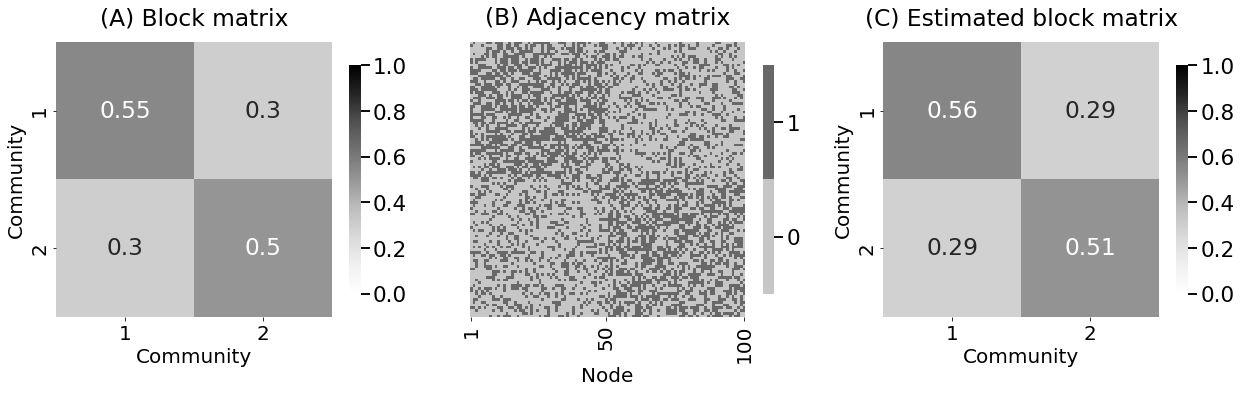
\includegraphics[width=\linewidth]{applications/ch7/Images/model_select_ex.png}
    \caption{\textbf{(A)} the true probability matrix underlying the $SBM_n(\vec z, B)$ random network, \textbf{(B)} a sample of the random network, \textbf{(C)} the estimated block matrix.}
    \label{fig:ch7:model:ex}
\end{figure}

\subsection{Model selection and random networks}

\textit{Model selection} is the task of selecting among several possible statistical models which we think may describe our sample. We do this using quantitative strategies to determine which statistical models are best supported by the data. 

\begin{floatingbox}[h]\caption{Model selection with coin flips}
\label{box:ch7:model:twosample_coin}
In Remark \ref{box:ch7:testing:twosample_coin}, we introduced a simple two-sample test for coin flip data. In this example, we wanted to determine whether the two coins had the same probability, or whether the probability was different. The null hypothesis was $H_0 : p_1 = p_2$, against $H_A : p_1 \neq p_2$. 

This example can also be thought of as a trivial example in model selection. In this case, we have two samples of data. While our question can be thought of as a two-sample test looking for a difference between the two samples, it can also be thought of as determining whether or not there were really two-samples of data in the first place.

Notice that under our null hypothesis, we are basically asking whether a coin with the same probability was used for both of the samples. Under the alternative hypothesis, we are basically asking whether two fundamentally different coins were used for each of the samples.

So, the null can be reformulated as: can the two samples be described using the same probability term, or can the two samples be best described using different probability terms. Stated another way, does the most reasonable model for the data have one parameter (the same probability term, for both samples), or should we describe it with two parameters (a unique probability term for each sample)?
\end{floatingbox}

In Remark \ref{box:ch7:model:twosample_coin}, we introduce the idea of model selection as it relates to a simple question of whether a collection of twenty coin flips (from two samples of data) should be described using a single probability term for all twenty coin flips, or whether each of the ten coin flips should be described using two probability terms.

In much the same light, we can formulate our block matrices under the same light. Remember that the block matrix for a simple $SBM_n(\vec z, B)$ random network is organized as:
\begin{align*}
    B &= \begin{bmatrix}
        b_{11} & b_{12} \\
        b_{12} & b_{22}
    \end{bmatrix}.
\end{align*}
The symmetry of $B$ is because the underlying simple random network is undirected (so $b_{21} = b_{12}$). What we want to do formally is ask, does the data provide us with enough evidence to support that the homophilic network is not a planted partition (does $b_{11} \neq b_{22}$)? Further, is there really any reason to believe that there is any block structure to it, at all?

If we only had the estimated block matrix in Figure \ref{fig:ch7:model:ex}(C), it feels immediate that we could conclude that the network is homophilic, but ``it feels immediate'' is not particularly quantitative.

As we move to more and more complicated models, there is concurrently a tradeoff known as model parsimony. \textit{Model parsimony} is the idea that simpler models with fewer parameters that describe are generally preferable to more complicated models with more parameters, provided both models describe the data equally well. This idea ties directly into the bias/variance tradeoff, which we discussed in Section \ref{sec:ch4:regularization}.

This can be interpreted with a level of rigor by considering the extremes. In the simplest case, we could have a random network model with a single parameter (an $ER_n(p)$ random network). On the other end of the spectrum, we have the most complicated model, which is an $IER_n(P)$ random network with a unique probability term $p_{ij}$ for each edge. 

The idea is that, with most datasets, we can find a ``happy medium'' somewhere in between, wherein the model is complicated enough that it describes our system faithfully, but not so complicated that we end up overfitting when we use our network sample to analyze it. Through model selection, we attempt to develop principled strategies that allow us to favor parsimonious models that are complicated enough to describe the data efficiently, but not so complicated that our data cannot support the downstream conclusions that we develop. 

\subsubsection*{Sequentially nested hypotheses}

A critical feature that we will exploit for model selection with $2 \times 2$ block matrices is the idea that we have nested hypotheses. A hypothesis $H_1$ is \textit{nested} in another hypothesis $H_2$ if, whenever $H_2$ is true, $H_1$ is true too. 

In the coin flip example, we can reformulate our two hypotheses $H_0$ and $H_A$ as a sequence of nested hypotheses. Notice that if $H_0$ is true, the model could be described with a single probability term $p_1 = p_2 = a$. On the other hand, if $H_A$ is true, the model can be described by $p_1 = b$ and $p_2 = c$. That $H_A$ is nested in $H_0$ would mean that even if we use two numbers $b$ and $c$ as the probabilities of $p_1$ and $p_2$, we could always just set $b = c$, and end up with the model in $H_0$. If in the underlying system it is the case that $p_1 \neq p_2$ (and $H_A$ is true), then we really need that additional delineation of terms $b$ and $c$. On the other hand, if in the underlying system it is the case that $p_1 = p_2$, we can get away with just the one term. 

\paragraph*{Developing sequentially nested hypotheses for network data}

To consider this idea of sequentially nested hypotheses for network data, let's think about the setting that we have with our $2 \times 2$ block matrix. In this case, we have three groups of edges: 
\begin{enumerate}
    \item the group of edges where both nodes are from community one,
    \item the group of edges where both nodes are from community two, and 
    \item the group of edges where one node is from community one and the other from community two.
\end{enumerate}
For each edge, we can build an edge group assignment matrix, which re-conceptualizes our $SBM_n(\vec z, B)$ random network as a $SIEM_n(D, \vec p)$ random network. We will still study the problem :

\begin{lstlisting}[style=python]
D = np.array(zs).reshape(n, 1) @ np.array(zs).reshape(1, n)
D[D == 4] = 3
\end{lstlisting}

This gives us three ``samples'' (to borrow the analogy from our coin flip model) of data. Visually, it seems pretty evident that the model is probably homophilic, so this motivates the following sequentially nested hypotheses:
\begin{enumerate}
    \item $H_0$: The block matrix is Erd\"os-R\'enyi, where $b_{11} = b_{12} = b_{22} = a$.
    \item $H_1$: The block matrix is a homophilic planted partition, where $b_{11} = b_{22} = a$, but $b_{12} = b$, and $a > b$. Note that this hypothesis is nested in $H_0$, as $H_0$ would be true if we were to choose $b$ where $a = b$.
    \item $H_2$: The block matrix is homophilic with heterogeneous on-diagonal blocks, where $b_{11} = a$, $b_{12} = b$, and $b_{22} = c$, where $b_{11}, b_{22} > b_{12}$. Note that this hypothesis is nested $H_1$, as $H_1$ would be true in a choice of $c$ where $a = c$.
\end{enumerate}


\paragraph*{Testing sequentially nested hypotheses}

The first question that you might have is how we can actually determine which of these sequentially nested hypotheses to pick. Remember that in the two hypothesis case, we tested the null hypothesis against the alternative hypothesis. In this case, however, we have three hypotheses, so we need a slightly different strategy. 

Since we already have strategies for testing two hypotheses, statisticians have come up with a simple but remarkably elegant solution to this problem. Basically, the idea is that we start with the simplest model that we could have ($H_0$). We add a single layer of complexity in the scope of the models that we think could be reasonable ($H_1$), and simply test $H_0$ as the null hypothesis against $H_1$ as the alternative hypothesis. 

Intuitively, the idea is that for a sequence of nested hypotheses with $N$ levels, for a hypothesis at level $n$ to be reasonable, then the hypothesis at level $n-1$ has to be more reasonable than the one at level $n-2$ first. In our case, this amounts to determining that if the model has a homophilic block matrix with a heterogeneous on-diagonal block structure, we should probably first know whether a homophilic block matrix makes sense in the first place. We basically follow this pattern backwards, which leads to the insight that it makes sense to begin at $H_0$ against $H_1$.

Once we test $H_0$ against $H_1$, we have two routes: either the data does not support $H_0$ and we reject $H_0$, or we do not have evidence to reject $H_0$. If we do not have evidence to reject $H_0$, we stop with the idea that we want to, in some sense, only move to complicated models when strictly necessary (e.g., when the data does not support the simpler model). We repeat this process over and over again, in the process known as \textit{forwards model selection}, in Algorithm \ref{alg:ch7:forwards}.

\begin{algorithm}[h]\caption{Forwards model selection}
\label{alg:ch7:forwards}
\KwData{$H_1, H_2, \hdots, H_N$ a sequence of sequentially nested hypotheses delineating different models to describe the data.}
\KwResult{The deepest hypothesis that is not rejected against the next sequential alternative.}
\SetAlgoLined

Set $n = 1$, and \texttt{stop=False}.

\While{\texttt{stop = False}} {
    
    Test $H_{n-1}$ as the null hypothesis against $H_n$ as the alternative hypothesis. 
    
    \uIf{no evidence to reject $H_{n-1}$\text{ or }$n = N - 1$} {
        Let \texttt{stop=True}.
    } \Else {
        Let $n = n + 1$.
    }
}

\Return{$H_n$}
\end{algorithm}

\subsection{Applying sequentially nested hypotheses to network data}

Remember with network data, the network samples have binary adjacency matrix entries $a_{ij}$ (which take values of $0$ or $1$). Remember that when we had two samples of data, a suitable representation was the contingency table in Table \ref{tab:ch7:testing:cont}. When we have three samples of binary data, what else can we use?

The best way to summarize this data is identical to that which we used for the two-class case: another contingency table. The contingency table for a $3$-sample example is lain out in Table \ref{tab:ch7:model:cont}.

\begin{table}[h]
    \centering
    \begin{tabular}{c | c|c|c}
         & Edge-group $1$ & Edge-group $2$ & Edge-group $3$ \\
         \hline
         Number of edges with $a_{ij} = 1$ & &  & \\
         Number of edges with $a_{ij} = 0$ & &  &
    \end{tabular}
    \caption{A contingency table with three samples.}
    \label{tab:ch7:model:cont}
\end{table}

In the two-sample case with $2$ columns, the Fisher's exact test is generally regarded as the preferred statistical test, however that only works with two samples (and not three). For this reason, we turn to the $\chi$-squared test, discussed briefly in Remark \ref{box:ch7:model:chisq}.

\begin{floatingbox}[h]\caption{The $\chi$-squared test for $2 \times K$ contingency tables}
\label{box:ch7:model:chisq}
When you have contingency tables with $K$ columns and $2$ rows, a good technique is known as the $\chi$-squared test. Unlike the Fisher's exact test, the $\chi$-squared test is an asymptotic test, in that it is effective when we have many samples of data, but has limitations when we do not have many samples of data. While it is generally preferable to defer to exact tests when possible, it will do for our purposes here. 

This statistical test gives us a test statistic, $X$, which is larger when the $K$ groups differ more, and small when the $K$ groups are the same. We use properties about the underlying network (that the edges are independent) to deduce what $X$ should look like if the $K$ groups are the same (known as the $\chi$-squared distribution). Finally, we obtain a $p$-value for our test by studying how anamalous the test statistic $X$ that we observed is compared to the $\chi$-squared distribution.
\end{floatingbox}

\begin{comment}
Without going into too much technical depth, the $\chi$-squared test operates on $2 \times K$ contingency tables and produces a number (the $\chi$-squared test statistic) which tends to be large when the $K$-way groupings differ, and tends to be small when the $K$-way groupings do not differ. 

This allows us to test whether, if $p_k$ are the column-wise mean probabilities for each of the $K$ levels, $H_0 : p_1 = p_2 = \hdots p_K$ against $H_A : p_k \neq p_l$ for some $k, l$. In words, it gives us a way to generalize the Fisher's exact test procedure to determine whether all of the columns have the same probability or whether some of the columns have different probabilities. 

Crucially, if we run two $\chi$-squared tests corresponding to two different table groupings with nested alternative hypotheses, we can compare the $\chi$-squared statistics (across the two different table groupings) and determine which grouping is more appropriate. 
\end{comment}

To refer back to our sequentially nested hypotheses, we can test whether the block model is Erd\"os-R\'enyi against whether it is homophilic planted partition directly, using the $2 \times 2$ contingency table in Table \ref{tab:ch7:model:cont_homo}. This produces a test statistic $X^{(1)}$, which we can use to test $H_0$ that the model is Erd\"os-R\'enyi against $H_A$ that the model is a homophilic planted partition. 

\begin{table}[h]
    \centering
    \begin{tabular}{c|c|c}
         & $(1, 1)$ and $(2, 2)$ blocks & $(1, 2)$ block \\
         \hline
         Number with $a_{ij} = 1$ & & \\
         Number with $a_{ij} = 0$ & & 
    \end{tabular}
    \caption{Contingency table for testing whether a block model is Erd\"os-R\'enyi against whether it is homophilic planted partition.}
    \label{tab:ch7:model:cont_homo}
\end{table}

In our data, the first step is to establish a model with the desired contingency table. We do this by using a \texttt{pandas} dataframe where the rows are edges, the firstcolumn indicates the value of the adjacency matrix for that particular edge, and the second column indicate the edge-group. Then, we indicate the \texttt{python} that we would like a statistical model for binary data by indicating a logistic regression with the \texttt{statsmodels} package:

\begin{lstlisting}[style=python]

\end{lstlisting}

Next, we run a second test, using the contingency table in Table \ref{tab:ch7:model:cont_het}. This produces a test statistic $X^{(2)}$, which we can use to test $H_0$ that the model is not homophilic with heterogeneous on-diagonal blocks against $H_A$ that the model is homophilic with heterogeneous on-diagonal blocks. 

\begin{table}[h]
    \centering
    \begin{tabular}{c|c|c|c}
         & $(1, 1)$ block & $(1, 2)$ block & $(2, 2)$ block \\
         \hline
         Number with $a_{ij} = 1$ & & & \\
         Number with $a_{ij} = 0$ & & & 
    \end{tabular}
    \caption{Contingency table for testing whether a block model is Erd\"os-R\'enyi against whether it is homophilic planted partition.}
    \label{tab:ch7:model:cont_het}
\end{table}

The magic occurs here: when we look at the ratio $\frac{X^{(2)}}{X^{(1)}}$, the test that we are really running when the hypotheses are sequentially nested is a test of whether $H_0$ the model is a homophilic planted partition against $H_A$ that the model is homophilic with heterogeneous on-diagonal blocks. This strange result occurs because, when the hypotheses are nested, we can describe what $\frac{X^{(2)}}{X^{(1)}}$ looks like if the more complicated model does not add any value to the simpler model. Whereas the reference before was the $\chi$-squared distribution, the reference here is known as the $F$-distribution. 

This procedure is generally known as an \textit{Analysis of Variance} (ANOVA), and is extremely common when comparing $K$ groups of data in both binary and non-binary situations. In our case, our network samples have adjacency matrix entries with binary values ($0$ or $1$), so we can use it.

\begin{lstlisting}[style=python]

\end{lstlisting}

\newpage
\section{The vertex nomination problem}
\label{sec:ch7:vn}

As we learned in Section \ref{sec:ch5:sbm} and have reinforced throughout this book, the $SBM_n(\vec z, B)$ random network is a useful conceptual model for many network presentations that we might come across in real data. Problematically, in many applications, this conceptual model cannot be directly applied, as it is often the case that we do not have node covariates that we can use to group nodes into communities, or we have many node covariates and are not sure which impact the connection probabilities within the network. When this was the case, we learned that we could spectral embed with techniques from Chapter \ref{sec:ch6}, and then use strategies like community detection from Section \ref{sec:ch7:comm_detect} to estimate community structure from the network. 

In some applications, your data will fall somewhere in between: you might know the communities of some nodes, but you might be unaware of the communities for others. The \textit{vertex nomination} problem is to identify a set of nodes without a community assignment, which are maximally similar to a set of nodes for which you have a community assignment \cite{Fishkind2015Sep}. Our goal is to produce a \textit{nomination list}, which is a set of unlabeled nodes which are most likely to be similar to the labeled nodes. In Remark \ref{box:ch7:vn:ex}, we detail a case study of the vertex nomination problem in practice.

\begin{floatingbox}[h]\caption{Human trafficking and the vertex nomination problem}
\label{box:ch7:vn:ex}
One of the most important jobs for law enforcement officers is to maintain an understanding of the business dealings of criminals. In recent years, the internet has become a popular medium for sharing and organizing illicit activity. The Department of Defense released the Memex tool, which facilitates precise searches over isolated web domains. 

This has allowed investigators to develop a network with tens of thousands of nodes \cite{Fishkind2019Mar,Yoder2018Feb}, which represent individual web pages for job postings on the internet. An edge exists between a pair of nodes if the contact information (phone number) or the region (city) on the contact information is the same. A small number of nodes in the network were identified directly as being tied to human trafficking through the content on the webpage or the URL itself. The goal is to produce the set of remaining nodes for which the human trafficking status is unknown which are most likely to be tied to human trafficking, so that the postings can be further monitored and investigated by law enforcement. 
\end{floatingbox}

For this section, we'll imagine that we have an $SBM_n(\vec z, B)$ random network with $n=1000$ nodes representing web pages, of which the community of each node will represent whether or not the web page is associated with human trafficking. $50$ will be associated with human trafficking and $950$ will not be associated with human trafficking. Of the $50$ web pages associated with human trafficking, we will only know the community label for $20$ of them. 

\begin{lstlisting}[style=python]
import numpy as np
from graspologic.simulations import sbm

ns = [50, 950]

A = sbm(ns, p=np.array([[0.3, 0.1], [0.1, 0.2]]))
\end{lstlisting}

Figure \ref{fig:ch7:vn:ex}(A) shows a plot of the adjacency matrix, with the nodes organized by community. 



The nomination task here isn't just classification: it's prioritization. Of the remaining $980$ web pages, we want to produce a list of the remaining nodes, which are organized in the order which we should prioritize them for further investigation. If we are successful, the nomination list that we propose should generally contain the remaining $30$ nodes in the human trafficking community as the highest priority, and the $950$ nodes unassociated with human trafficking as lower priority.


\subsection{The seed nodes}

The key idea for addressing the vertex nomination problem is the use of seed nodes. A \textit{seed node} is a node in a network for which you have information that you know to be true. 

In this case, we know the node labels for $20$ of the human traffickers. We will assume here that the seed nodes are randomly assigned amongst the $20$ human traffickers.

\begin{lstlisting}[style=python]
# the number of seed nodes
nseeds = 20
# The first ns[0] nodes are the human traffickers, so choose 20 seeds
# at random
seed_ids = np.random.choice(ns[0], size=20)
\end{lstlisting}

\subsection{Spectral vertex nomination (\texttt{svn})}


The first step to spectral vertex nomination is to use a spectral embedding to obtain estimated latent positions. We can do this with \texttt{ase}:

\begin{lstlisting}[style=python]
from graspologic.embed import AdjacencySpectralEmbed as ase

Xhat = ase().fit_transform(A)
\end{lstlisting}

In Figure \ref{fig:ch7:vn:ex}(B), the estimated latent positions for the seed (the web pages confirmed to be associated with human trafficking, in red) and non-seed (for which the human trafficking status is unknown, in black) nodes are shown. Based on what you know from Section \ref{sec:ch6:ase} and \ref{sec:ch7:comm_detect}, nodes which are in the same community tend to also have similar estimated latent positions. This was a consequence of the fact that the underlying latent positions are identical for nodes in the same community, which you learned in Section \ref{sec:ch5:psd_block:same_lp}. 

\begin{figure}[h]
    \centering
    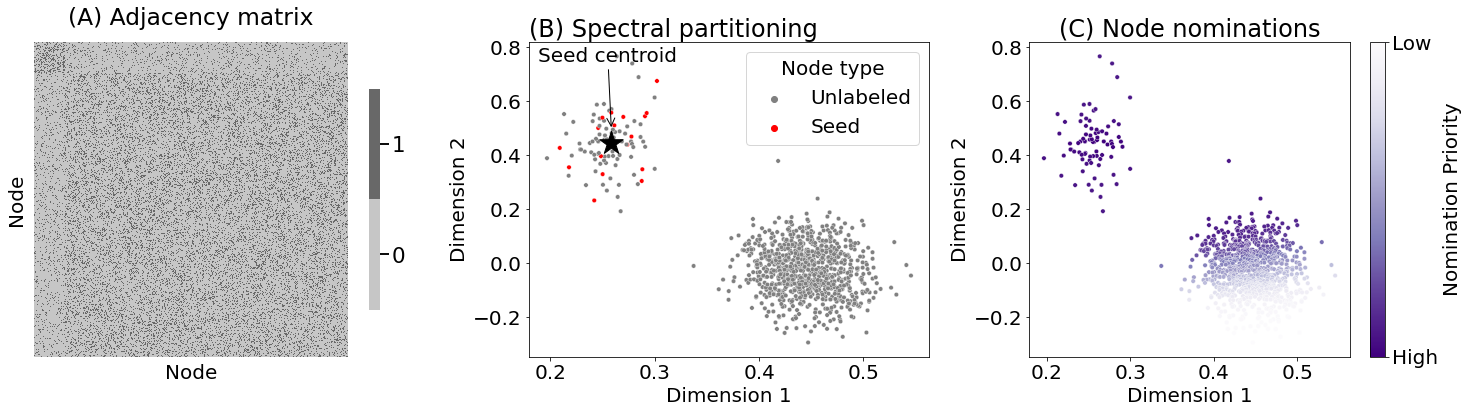
\includegraphics[width=\linewidth]{applications/ch7/Images/vn.png}
    \caption[Web page network for vertex nomination.]{\textbf{(A)} The adjacency matrix for the web page network. \textbf{(B)} the estimated latent positions for the nodes in the web page network (faint points). The centroid of the seed nodes is annotated directly. \textbf{(C)} the nomination priorities for each of the unlabelled nodes. Nodes which are closer to the seed centroid have higher priority.}
    \label{fig:ch7:vn:ex}
\end{figure}

Back in Section \ref{sec:ch6:ase}, we used the Euclidean distance from Remark \ref{def:ch6:se:eucl_dist} to quantify what we meant by nodes from the same community having ``similar'' estimated latent positions. Remember that when we used \texttt{KMeans} to estimate the unknown community assignments in Section \ref{sec:ch7:comm_detect}, the key idea was that we could exploit the fact that nodes in the same community had similar latent positions to identify clusters of nodes which had similar latent positions. This resulted in community-specific mean vectors $\vec \mu_k$, and we assigned points to communities depending on their proximity to the community-specific mean vectors.

Here, we will use a similar insight. We already know the community assignments for the seed vectors in our community of interest, and all nodes $i$ from the same community have the same underlying latent position $\vec x_i$. This property does not hold in the estimated latent positions $\hat{\vec x}_i$ for the nodes in the same community, since the latent positions are imperfectly estimated, which we learned from Section \ref{sec:ch6:ase}.

Since the underlying latent positions of the random network are the same, a reasonable estimated latent position for the community can be obtained by performing a spectral clustering (via \texttt{KMeans}, like we did in Section \ref{sec:ch7:comm_detect}):

\begin{lstlisting}[style=python]
from graspologic.embed import AdjacencySpectralEmbed as ase
from sklearn.cluster import KMeans
from graphbook_code import ohe_comm_vec

Xhat = ase().fit_transform(A)
# community detection with kmeans
km_clust = KMeans(n_clusters=2)
km_clust.fit(Xhat)
labels_kmeans = km_clust.fit_predict(Xhat)
\end{lstlisting}

For each seed node, we can obtain the a surrogate for the estimated latent position associated with the community of the seeds by simply finding which of the communities the seeds tended to be assigned to, and then using the centroid associated with this community to find nodes most similar to the seed nodes:

\begin{lstlisting}[style=python]
# estimated community assignment matrix
Chat = ohe_comm_vec(labels_kmeans)

# get the community (class) with the most seeds
comm_of_seeds = np.argmax(Chat[seed_ids,:].sum(axis=0))

# get centroid of the community that seeds tend to be
# assigned to
centroid_seeds = km_clust.cluster_centers_[comm_of_seeds]
\end{lstlisting}

The centroid of the community that the most seed nodes were assigned to is indicated in Figure \ref{fig:ch7:vn:ex}(B), by the large red star. 

Finally, using the Euclidean distance, we can estimate the spatial proximity for each unlabeled node to the centroid that the most the seed nodes were assigned to. We will use this spatial proximity to the centroid as a surrogate for unlabeled nodes being ``similar'' to the seed nodes in producing our nomination list:

\begin{lstlisting}[style=python]
from scipy.spatial.distance import cdist
from scipy.stats import rankdata

# compute the distance to the centroid for all estimated latent positions
dists_to_centroid = cdist(Xhat, centroid_seeds.reshape(1, -1)).reshape(-1)
# compute the node numbers for all the nonseed nodes
nonseed_bool = np.ones((np.sum(ns)))
nonseed_bool[seed_ids] = 0
nonseed_ids = np.array(np.where(nonseed_bool)).reshape(-1)

# isolate the distances to the centroid for the nonseed nodes
nonseed_dists = dists_to_centroid[nonseed_ids]
\end{lstlisting}

To produce the nomination list, we can sort the distances of the nonseed nodes to the centroid, return the index-sorted ordering, and then output our nomination list by using reordering the nonseed indices in order of their distances. The following code will do just this for us:


\begin{lstlisting}[style=python]
# produce the nomination list
nom_list_nonseeds = np.argsort(nonseed_dists).reshape(-1)
# obtain a nomination list in terms of the original node ids
nom_list = nonseed_ids[nom_list_nonseeds]
\end{lstlisting}

In Figure \ref{fig:ch7:vn:ex}(C), we color the unlabeled nodes (which were gray in Figure \ref{fig:ch7:vn:ex}(B)) by their spatial proximity to the seed centroid. Note that the unlabelled nodes which are closest to the seed centroid tend to have higher spatial proximities, and are hence higher priority in the nomination list (with a smaller numerical label in \texttt{nom\_list}).

This procedure is known as the ``Spectral Partitioning Nomination Scheme'', or \texttt{sp}, and has been studied in several areas of application \cite{Fishkind2015Sep,Yoder2018Feb}.

\subsection{Extensions to other problems}

There are a large number of ways that we could have approached the vertex nomination problem differently. Let's take a look at a few of them.None of these approaches are ``better'' or ``worse'', than others, and it is important to highlight that each can be leveraged to answer a different network learning question \cite{Coppersmith2012Jan,Coppersmith2014Mar,Yoder2018Feb,Fishkind2015Sep,Fishkind2019Mar}. When you have a vertex nomination problem, you will likely have to tailor the strategy to your network data.


\paragraph*{Different strategies for spectral partitioning}

We presumed that our network had two communities, and two embedding dimensions, which was largely a function of visual simplicity when viewing the node nominations in Figure \ref{fig:ch7:vn:ex}(C). However, there is no reason we need to necessarily assume the number of communities or the ahead of time, and we could just as easily have used dimensionality selection as in Section \ref{sec:ch6:dimest:dimselect}, automated the community selection procedure like we did in Section \ref{sec:ch7:comm_detect}, or substituted different clustering algorithms and different notions of similarity.

For instance, a popular choice for community detection in \cite{Yoder2018Feb} is \texttt{GMM}, where the notion of similarity is the probability density of a particular unlabeled point given the mean and variance of the cluster the most seeds are assigned to. This enables robustness to networks where the underlying random network is $DCSBM_n(\vec z, \vec \theta, B)$, which you learned in Section \ref{sec:ch7:comm_detect}.

\paragraph*{Extending spectral partitioning to related problems}

The spectral partitioning nomination scheme can be extended directly to many other related problems. A key limitation here is that we are presuming that our nodes are in one of two groups, and all of the labeled nodes that we pass in are associated with the same group. Our goal is to prioritize nodes that are likely to also be from that same group. 

On the other hand, we could have just as easily identified nomination lists on a per-seed-node basis; e.g., for each seed node, we could have found a set of unlabeled nodes that have spatially proximal estimated latent positions. This extension provides the intuitive foundation for the \textit{graph matching problem} \cite{Fishkind2015Sep, Fishkind2019Mar}, which you will learn about in Section \ref{sec:ch8:gm}.

\paragraph*{We could have ignored partitioning techniques entirely}

We could have ignored partitioning and latent community detection approaches entirely, and simply estimated the ``centroid'' directly by taking the average estimated latent position of all of the seed nodes.

\newpage
\section{Out-of-sample embedding}
\label{sec:ch7:oos}

While the networks that we have been using in this book have generally been on the small side, for larger networks, computing embeddings can be expensive. In Remark \ref{box:ch7:oos:ex}, we detail an example of why this is the case.

\begin{floatingbox}[h]\caption{Spectral embeddings of networks with many nodes}
\label{box:ch7:oos:ex}
Let's imagine that you have a network, where the nodes are web pages and the edges are whether a pair of web pages cross-link to one another. There are $n=10^9$ nodes in the network, and let's imagine that you have a strong suspicion that there are communities that are homophilic (they have high within-community clustering). For any given day, you want to have a record of the estimated communities that exist in your network. Procedurally, we learned how to address this task in Section \ref{sec:ch7:comm_detect}: you begin by embedding the network, and then you train an unsupervised classifier to identify estimated community structure from the estimated latent positions.

The next day, however, you have a problem: another $n'=5$ web pages were added to the network. Being a diligent machine learning scientist, you could simply re-execute your procedure you used the previous day. However, this has a limitation: the \texttt{svd} (a crucial component of spectral embeddings), while more than sufficient for the networks that we have been working with in this book, does not scale particularly well to large networks. The \textit{time complexity} refers to the amount of time that it takes an algorithm (in the worst case) to yield a solution, and the \textit{space complexity} refers to the amount of RAM that the computer would need to access to yield a solution. When working with large networks and using complicated algorithms, the time and space complexity will be problems that we will need to contend with. If you are unfamiliar with time and space complexity, we would recommend that you review \cite{Banerjee2021Dec}.

The \texttt{svd} tends to scale in $\mathcal O(n^3)$ time, and the space requirements are no better, scaling at about $\mathcal O(n^2)$. This means that for networks with more nodes, embedding the network will take a lot of computing time and space to calculate. Your web pages network is very large, so this could get expensive very quickly!
\end{floatingbox}

The key problem is that the network is extremely large, and the \texttt{svd} (and consequently, the \texttt{ase}) scales remarkably poorly for large networks. When you embed large networks, you might have to resort to using special super computers with enormous numbers of cores or memory to get the results that you need. These computers tend to be expensive, so the cost of this operation could skyrocket quickly. 

Remember that when we make assumptions that our network $A$ is a sample from an underlying random network $\mathbf A$ as in Section \ref{sec:ch6:ase:whyuse}, the estimates of latent positions produced by \texttt{ase} tend to be fairly close estimates of the true underlying latent positions in the network. Further, as the network grows, these estimates get better and better. This means that if we embedded a network with $n + n'$ nodes, the embedding is probably going to be fractionally better than the embedding if we just used $n$ nodes. 

The difference, however, will not be particularly substantial, and sometimes we might be willing to take a slight loss in the precision of our estimates at the tradeoff of having far greater computational and algorithmic efficiency. In these cases, we can use an \textit{out of sample embedding}, or \texttt{oose} \cite{Levin2018Jul,Bengio2003}, to embed new nodes (the ``out-of-sample'' nodes) in an existing latent space computed using only the original nodes (the ``in-sample'' nodes). 

When we do this, we obtain estimated latent positions for our new nodes in a shared space between the new and old nodes. While we might still want to recompute the full embedding occassionally, in the short term we can save a lot of computation resources (which can mean time, money, and effort) and still obtain estimated latent positions that are good enough for our downstream analysis.

\subsection{\texttt{oose} requires a full adjacency matrix and adjacency vectors for each new node}

Let's begin by generating a network. For the out-of-sample embedding, we first need an $n$-node network (the ``in-sample'' nodes). The crucial ingredient that we will need for the out-of-sample nodes are instructions that tell us how the out-of-sample nodes are connected to the ``in-sample'' nodes. This is accomplished via adjacency vectors, which can be thought of as behaving a lot like ``rows'' of an adjacency matrix. An \textit{adjacency vector} for a node $j$ in relation to an $n$-node network is a length-$n$ vector $\vec a_j$, where $a_{ij}$ indicates whether node $i$ and node $j$ are connected.

For demonstration purposes, we'll generate a sample from an $SBM_n(\vec z, B)$ random network with $n + n'$ nodes. The in-sample nodes will be $50$ nodes from community $1$, and $50$ nodes from community $2$. The out-of-sample nodes will be $1$ node from community $1$, and $2$ nodes from community $2$:

\begin{lstlisting}[style=python]
import numpy as np
from graspologic.simulations import sbm

# the in-sample nodes
n = 100
nk = 50
# the out-of-sample nodes
np1 = 1; np2 = 2
B = np.array([[0.6, 0.2], [0.2, 0.4]])
# sample network
A, zs = sbm([nk + np1, nk + np2], B, return_labels=True)
\end{lstlisting}

Next, we will remove the $n'$ ``out-of-sample'' nodes with \texttt{graspologic}. This will give us an $n \times n$ adjacency matrix corresponding to the subnetwork induced by the in-sample nodes, and an $n \times n'$ matrix $A'$ of adjacency vectors, which indicate the connectivity of out-of-sample nodes to in-sample nodes:

\begin{lstlisting}[style=python]
from graspologic.utils import remove_vertices

# the indices of the out-of-sample nodes
oos_idx = [nk, nk + np1 + nk, nk + np1 + nk + 1]
# get adjacency matrix and the adjacency vectors A prime
Ain, Ap = remove_vertices(A, indices=oos_idx, return_removed=True)
\end{lstlisting}

In Figure \ref{fig:ch7:oos:ex}(A), we plot the adjacency matrix of the in-sample nodes. Note the modular community structure. In Figure \ref{fig:ch7:oos:ex}(B), we show the adjacency vectors for each of the $3$ out-of-sample nodes, in relation to the in-sample nodes from Figure \ref{fig:ch7:oos:ex}(A). Further, notice that the out-of-sample nodes tend to follow the patterns from their respective communities; out-of-sample node $1$ is in community $1$, and tends to have more connections with nodes of community $1$. Out-of-sample nodes $2$ and $3$ are in community $2$, and tend to have more connections with nodes of community $2$.

\begin{figure}[h]
    \centering
    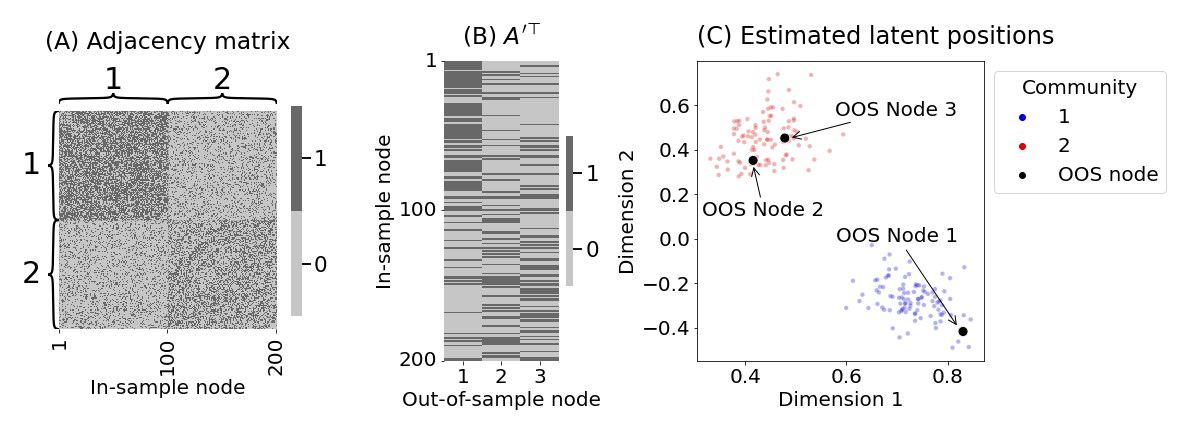
\includegraphics[width=\linewidth]{applications/ch7/Images/oos_ex.png}
    \caption[Out of sample embedding example]{\textbf{(A)} the adjacency matrix for the in-sample nodes. \textbf{(B)} the adjacency vectors (columns) for each of the $3$ out-of-sample nodes. \textbf{(C)} the estimated latent positions for each of the in-sample nodes (faint blue and red) with the estimated latent positions for the out-of-sample nodes (black).}
    \label{fig:ch7:oos:ex}
\end{figure}

\subsection{Conceptualizing the probability vector for an out-of-sample node}

If we add an out-of-sample node $j$ to the network, the adjacency matrix for this new network is:
\begin{align*}
    A &= \begin{bmatrix}
        A & \vec a_j \\
        \vec a_j^\top & 0
    \end{bmatrix}
\end{align*}

Where the $j$ simply denotes that we added the node $j$ to the network, and $\vec a_j$ is the adjacency vector for node $j$. If we assume that this new network is a sample from an $RDPG_{n+1}(X')$ random network, the latent position matrix is:
\begin{align*}
    X' &= \begin{bmatrix}
        \vec x_1^\top \\
        \vdots\\
        \vec x_n^\top \\
        \vec x_j^\top
    \end{bmatrix}
\end{align*}
where $\vec x_j$ is the latent position (the quantity that we want to obtain) associated with our out-of-sample node $j$.

Remember that for an $RDPG_{n+1}(X')$ random network, that for all pairs of nodes $i$ and $i'$, $p_{ii'} = \vec x_i^\top \vec x_{i'}$. Therefore, the matrix product $X\vec x_j$ is:
\begin{align*}
    X\vec x_j &= \begin{bmatrix}
        \vec x_1^\top \\
        \vdots \\
        \vec x_n^\top
    \end{bmatrix}\vec x_j = \begin{bmatrix}
        \vec x_1^\top \vec x_j \\
        \vdots \\
        \vec x_n^\top \vec x_j
    \end{bmatrix} = \begin{bmatrix}
        p_{1j} \\
        \vdots \\
        p_{nj}
    \end{bmatrix} = \vec p_{j},
\end{align*}
where we just used the standard rules of matrix multiplication for the second equality, and then used the definition of $p_{ij}$ for the in-sample nodes. We will call this vector $\vec p_{j}$ the probability vector of node $j$, which has entries $p_{ij}$ for all $n$ in-sample nodes. In particular, this implies that:
\begin{align*}
    X\vec x_j - \vec p_{j} = \vec 0 = \begin{bmatrix}
        0 \\
        \vdots \\
        0 
    \end{bmatrix}, \numberthis \label{eqn:ch7:oos:e1}
\end{align*}
where $\vec 0$ is the $n$-dimensional $0$ vector.

\subsection{Estimating the out-of-sample node's latent position}

Our goal is to obtain an estimate of $\vec x_j$. Note that in Equation \ref{eqn:ch7:oos:e1}, we have two unobserved quantities here, $X$ and $\vec p_j$ (the probability vector for the node $j$). 

\subsubsection*{Estimating the unobserved quantities}

\paragraph*{Estimating the latent positions of the in-sample nodes}
Under our given setup, if $\mathbf A$ is a random network, it's not much of a stretch to assume that the network of only the in-sample nodes is an $RDPG_n(X)$ random network. By the logic that we developed in Section \ref{sec:ch6:ase}, a reasonable approach would be to use the \texttt{ase} to estimate latent positions for the in-sample nodes. We can do this using \texttt{graspologic}, with:

\begin{lstlisting}[style=python]
from graspologic.embed import AdjacencySpectralEmbed as ase

oos_embedder = ase()
# estimate latent positions for the in-sample nodes
# using the subnetwork induced by the in-sample nodes
Xhat_in = oos_embedder.fit_transform(Ain)
\end{lstlisting}

The in-sample estimated latent positions are shown in Figure \ref{fig:ch7:oos:ex}(C), with the faint colored nodes. The estimated latent positions are as-described for the estimated latent positions of a two-community $SBM_n(\vec z, B)$ random network: two relatively homogeneous (in terms of the latent positions) clusters of nodes. Remember that this is a function of the fact that the latent positions for a $SBM_n(\vec z, B)$ random network are identical within-community as-per Section \ref{sec:ch5:psd_block:same_lp}, and the estimated latent positions are estimating the latent positions.

\paragraph*{Formulating a least-squares optimization problem to estimate the probability vector}

Next, we'll turn to estimating $\vec p_j$.

\begin{floatingbox}[h]\caption{Estimating probabilities}
\label{box:ch7:oos:probs}
In section \ref{sec:ch6:mle}, we covered a basic result from probability for finding maximum likelihood estimates for coin flips. Let's assume that you have a random coin $\mathbf y$. For our purposes, let's imagine that this coin lands on heads (a value of $1$) with probability $p$ and tails (a value of $0$) with probability $1 - p$.

If you flip the coin $m$ times and obtain samples of coin flips $y_i$, a reasonable estimate of the probability that the coin lands on heads is given by the maximum likelihood estimate (MLE):
\begin{align*}
    \hat p &= \frac{1}{m}\sum_{i = 1}^m y_i,
\end{align*}
which is simply the fraction of the $m$ coin flips that landed on heads. 
\end{floatingbox}

As a logical extension of Remark \ref{box:ch7:oos:probs}, if you had one coin flip, the MLE would just be the outcome of that coin flip. With an identical rationale, we estimate $\vec p_j$ using:
\begin{align*}
    \hat p_{ij} &= a_{ij}.
\end{align*}
We estimate the probability that the in-sample nodes nodes $i$ and the out-of-sample node $j$ are connected as the adjacency value $a_{ij}$ between them. Stated another way, we will estimate $\hat{\vec p}_j$ with $\vec a_j$.

$\hat X$ is only an estimate of $X$, and is also inexact, which you learned about in Section \ref{sec:ch6:ase:whyuse}. Likewise, it is extremely unlikely that $\hat p_{ij} = p_{ij}$; that is, estimating the probability that the in-sample node $i$ and the out-of-sample node $j$ are connected with a single observation from the adjacency vector is probably not going to give us a particularly exact solution.  

Next, we're going to use what we have established in Equation \eqref{eqn:ch7:oos:e1} to establish a least-squares optimization problem. You can read about least-squares regression in Remark \ref{box:ch7:oos:lsreg} for a quick refresher. For a more detailed overview, check out \cite{Geron2017Mar}.

\begin{floatingbox}[h]\caption{Ordinary least-squares (OLS) regression}
\label{box:ch7:oos:lsreg}
Through least squares regression, you observe $n$ samples $y_i$, along with a set of features $\vec x_i$, which is a $d$-dimensional feature vector for each sample $i$. Your goal is to identify a set of $d$ coefficients $\vec \beta$, where for all $n$ samples:
\begin{align*}
    \vec y = \begin{bmatrix}
        y_1 \\
        \vdots \\
        y_n
    \end{bmatrix}&= X \vec \beta = \begin{bmatrix}
        \leftarrow & \vec x_1^\top & \rightarrow \\
        & \vdots &  \\
        \leftarrow & \vec x_n^\top & \rightarrow 
    \end{bmatrix}\begin{bmatrix}
        \beta_1 \\
        \vdots \\
        \beta_d
    \end{bmatrix}.
\end{align*}
By subtracting $X\beta$ from both sides, we obtain that:
\begin{align*}
    \vec y - X\vec\beta &= \vec 0,
\end{align*}
Unfortunately, the samples are noisy in practice, So we are limited to getting a close approximation of each sample; e.g.:
\begin{align*}
    y_i - \vec x_i^\top \beta &= r_i,\text{ and consequently, }\vec y - X\beta = \vec r
\end{align*}
where $r_i$ is known as the residual or error associated with sample $i$ in the regression. The \textit{mean-squared error} is defined as:
\begin{align*}
    MSE(\vec \beta) &= \frac{1}{n}\sum_{i = 1}^n\left(r_i\right)^2 = \frac{1}{n}\|X\vec \beta - \vec y\|^2_2.
\end{align*}
Our goal is to find the choice of $\vec \beta$ that minimizes the mean-squared error. With a bit of calculus, the solution to this is given by the \textit{normal equations}:
\begin{align*}
    \hat{\vec \beta} &= (X^\top X)^{-1}X^\top \vec y.
\end{align*}
\end{floatingbox}

Since our estimates of $X$ via $\hat X$ and $\vec p_j$ via $\vec a_j$ are imperfect, when we plug these into Equation \ref{eqn:ch7:oos:e1}, our equation becomes:
\begin{align*}
    \hat X \vec x_j - \vec a_j = \vec e_j,
\end{align*}
where $\vec e_j$ is an $n$-dimensional error term. In an ideal world, $\vec e_j$ would be exactly the zero vector, but since we imperfectly estimated $X$ and $\vec p_j$ with $\hat X$ and $\vec a_j$, this will not be the case. For this reason, we turn to least-squares regression. 

Using the normal equations in Remark \ref{box:ch7:oos:lsreg}, the estimate of $\vec x_j$ that minimizes the mean-squared error is given by:
\begin{align*}
    \hat{\vec x}_j &= \left(\hat X^\top \hat X\right)^{-1}\hat X^\top \vec a_j.\numberthis \label{eqn:ch7:oos:lsoose}
\end{align*}
This estimate $\hat{\vec x}_j$ is known as the \textit{least squares out-of-sample embedding} the out-of-sample node $j$. 

In the general case when you have $n'$ out-of-sample nodes with adjacency vectors to the in-sample nodes, the least-squares out-of-sample embedding (least-squares \texttt{oose}) for the out-of-sample nodes can be found using the procedure in Algorithm \ref{alg:ch7:oose}.

\begin{algorithm}
\label{alg:ch7:oose}
\caption{Least-squares out-of-sample embedding (least-squares \texttt{oose})}
\KwData{An estimated latent position matrix $\hat X$ for the in-sample nodes. \newline
$A'$, wich is a $n \times n'$ matrix whose columns $\vec a_j$ indicate the adjacency vectors $\vec a_j$ for each of the $n'$ out-of-sample nodes with the in-sample nodes.}
\KwResult{$d \times n'$ matrix, whose columns indicate the estimated latent positions for each of the $n'$ out-of-sample nodes.}
\SetAlgoLined

Let $\hat X' = \left(\hat X^\top \hat X\right)^{-1}\hat X^\top A'$.

\Return{$\hat X'$}
\end{algorithm}

We can perform embed the least-squares \texttt{oose} using \texttt{graspologic}:

\begin{lstlisting}[style=python]
Xhat_oos = oos_embedder.transform(Ap)
\end{lstlisting}
The embedding for the out-of-sample nodes is shown in Figure \ref{fig:ch7:oos:ex}(C). Note that out-of-sample node $1$ was in community $1$, and has an estimated latent position near those of the in-sample nodes from community $1$. Likewise, the out-of-sample nodes $2$ and $3$ were in community $2$, and have estimated latent positions near the in-sample nodes from community $2$. In this sense, least-squares \texttt{oose} has preserved the relative homogeneity in the latent positions within-community for the out-of-sample nodes with respect to the in-sample nodes, without requiring the in-sample network to be re-embedded.

\subsection{Computational Considerations}

Adapting the result from Remark \ref{box:ch7:oos:ex}, the spectral embeddings require the \texttt{svd} for the new network with $n + n'$ nodes where the number of in-sample nodes $n$ greatly exceeds the number of out-of-sample nodes $n'$. The time complexity of the \texttt{svd} is $\mathcal O\left(n^3\right)$, and the space complexity is $\mathcal O\left(n^2\right)$. 

On the other hand, the least-squares solution in Algorithm \ref{alg:ch7:oose} has a time complexity of $\mathcal O\left(d^2 n\right)$. If the embedding is meaningful, the number of estimated latent dimensions is usually far less than the number of nodes. So this approach has far improved time scalability over re-embedding the entire network, because for networks with large numbers of nodes $n^3$ will be much larger than $d^2 n$.

Space wise, when the number of in-sample nodes exceeds the number of estimated latent dimensions and the number of out-of-sample nodes, the space complexity to solve the normal equations is $\mathcal O\left(dn\right)$. By the same logic as above, $dn$ is much less than $n^2$, so the normal equations can be solved with far less space than recomputing the embedding.

\newpage

\bibliographystyle{vancouver}
\bibliography{references}